\documentclass[a4paper,11pt]{book}
%\documentclass[a4paper,twoside,11pt,titlepage]{book}
\usepackage{listings}
\usepackage[utf8]{inputenc}
\usepackage[spanish]{babel}
\usepackage{listings}
\usepackage{subcaption}
\usepackage{minted}
\usepackage{rotating}
\usepackage{comment}

% Define Colors

% \usepackage[style=list, number=none]{glossary} %
%\usepackage{titlesec}
%\usepackage{pailatino}

\decimalpoint
\usepackage{dcolumn}
\newcolumntype{.}{D{.}{\esperiod}{-1}}
\makeatletter
\addto\shorthandsspanish{\let\esperiod\es@period@code}
\makeatother


%\usepackage[chapter]{algorithm}
\RequirePackage{verbatim}
%\RequirePackage[Glenn]{fncychap}
\usepackage{fancyhdr}
\usepackage{graphicx}
\usepackage{afterpage}

\usepackage{longtable}

\usepackage[pdfborder={000}]{hyperref} %referencia

% ********************************************************************
% Re-usable information
% ********************************************************************
\newcommand{\myTitle}{Título del proyecto\xspace}
\newcommand{\myDegree}{Grado en ...\xspace}
\newcommand{\myName}{Juan del Río Gómez (alumno)\xspace}
\newcommand{\myProf}{Oresti Baños Legrán (tutor1)\xspace}
\newcommand{\myOtherProf}{Miguel Damas (tutor2)\xspace}
%\newcommand{\mySupervisor}{Put name here\xspace}
\newcommand{\myFaculty}{Escuela Técnica Superior de Ingenierías Informática y de
Telecomunicación\xspace}
\newcommand{\myFacultyShort}{E.T.S. de Ingenierías Informática y de
Telecomunicación\xspace}
\newcommand{\myDepartment}{Departamento de ...\xspace}
\newcommand{\myUni}{\protect{Universidad de Granada}\xspace}
\newcommand{\myLocation}{Granada\xspace}
\newcommand{\myTime}{\today\xspace}
\newcommand{\myVersion}{Version 0.1\xspace}


\hypersetup{
pdfauthor = {\myName (email (en) ugr (punto) es)},
pdftitle = {\myTitle},
pdfsubject = {},
pdfkeywords = {palabra_clave1, palabra_clave2, palabra_clave3, ...},
pdfcreator = {LaTeX con el paquete ....},
pdfproducer = {pdflatex}
}

%\hyphenation{}

\usepackage[backend=biber, style=authoryear]{biblatex}
\bibliography{bibliografia}
\setlength{\bibitemsep}{0.5cm} % Adjust this value as needed


%\usepackage{doxygen/doxygen}
%\usepackage{pdfpages}
\usepackage{url}
\usepackage{colortbl,longtable}
\usepackage[stable]{footmisc}
%\usepackage{index}

%\makeindex
%\usepackage[style=long, cols=2,border=plain,toc=true,number=none]{glossary}
% \makeglossary

% Definición de comandos que me son tiles:
%\renewcommand{\indexname}{Índice alfabético}
%\renewcommand{\glossaryname}{Glosario}

\pagestyle{fancy}
\fancyhf{}
\fancyhead[LO]{\leftmark}
\fancyhead[RE]{\rightmark}
\fancyhead[RO,LE]{\textbf{\thepage}}
\renewcommand{\chaptermark}[1]{\markboth{\textbf{#1}}{}}
\renewcommand{\sectionmark}[1]{\markright{\textbf{\thesection. #1}}}

\setlength{\headheight}{1.5\headheight}

\newcommand{\HRule}{\rule{\linewidth}{0.5mm}}
%Definimos los tipos teorema, ejemplo y definición podremos usar estos tipos
%simplemente poniendo \begin{teorema} \end{teorema} ...
\newtheorem{teorema}{Teorema}[chapter]
\newtheorem{ejemplo}{Ejemplo}[chapter]
\newtheorem{definicion}{Definición}[chapter]

\definecolor{gray97}{gray}{.97}
\definecolor{gray75}{gray}{.75}
\definecolor{gray45}{gray}{.45}
\definecolor{gray30}{gray}{.94}
\definecolor{skyblue6}{rgb}{.2, .6, .8}
\definecolor{blueice}{rgb}{.85, .96, .94}

\lstset{ frame=Ltb,
     framerule=0.5pt,
     aboveskip=0.5cm,
     framextopmargin=3pt,
     framexbottommargin=3pt,
     framexleftmargin=0.1cm,
     framesep=0pt,
     rulesep=.4pt,
     backgroundcolor=\color{gray97},
     rulesepcolor=\color{black},
     %
     stringstyle=\ttfamily,
     showstringspaces = false,
     basicstyle=\scriptsize\ttfamily,
     commentstyle=\color{gray45},
     keywordstyle=\bfseries,
     %
     numbers=left,
     numbersep=6pt,
     numberstyle=\tiny,
     numberfirstline = false,
     breaklines=true,
   }
 
% minimizar fragmentado de listados
\lstnewenvironment{listing}[1][]
%{\lstset{#1}\pagebreak[0]}{\pagebreak[0]}


\lstdefinestyle{CodigoC++}
   {
	basicstyle=\small,
	frame=single,
	backgroundcolor=\color{gray30},
	language=C++,
	numbers=left
   }

 
\lstdefinestyle{Consola}
   {basicstyle=\scriptsize\bf\ttfamily,
    backgroundcolor=\color{gray30},
    language=Python,
    frame=single,
    numbers=none,
   }

   \lstset{style=Consola}


\newcommand{\bigrule}{\titlerule[0.5mm]}


%Para conseguir que en las páginas en blanco no ponga cabecerass
\makeatletter
\def\clearpage{%
  \ifvmode
    \ifnum \@dbltopnum =\m@ne
      \ifdim \pagetotal <\topskip
        \hbox{}
      \fi
    \fi
  \fi
  \newpage
  \thispagestyle{empty}
  \write\m@ne{}
  \vbox{}
  \penalty -\@Mi
}
\makeatother

\usepackage{pdfpages}
\begin{document}
\begin{titlepage}
 
 
\newlength{\centeroffset}
\setlength{\centeroffset}{-0.5\oddsidemargin}
\addtolength{\centeroffset}{0.5\evensidemargin}
\thispagestyle{empty}

\noindent\hspace*{\centeroffset}\begin{minipage}{\textwidth}

\centering

\includegraphics[width=0.9\textwidth]{imagenes/logo_ugr.jpg}\\[1.4cm]

\textsc{ \Large TRABAJO FIN DE GRADO\\[0.2cm]}
\textsc{ GRADO EN INGENIERIA INFORMÁTICA }\\[1cm]
% Upper part of the page
% 
% Title
{\Huge\bfseries POSTCOVID-AI TelegramBot\\
}
\noindent\rule[-1ex]{\textwidth}{3pt}\\[3.5ex]
{\large\bfseries Facilitating data collection of people level human behavior\\
}
\end{minipage}

\vspace{1cm}
\noindent\hspace*{\centeroffset}\begin{minipage}{\textwidth}
\centering

\textbf{Autor}\\ {Juan del Río Gómez}\\[2.5ex]
\textbf{Directores}\\
{Oresti Baños Legrán \\
Miguel Damas Hermoso}\\[1.5cm]

\includegraphics[width=0.6\textwidth]{imagenes/etsiit_logo.png}\\[0.1cm]
\textsc{Escuela Técnica Superior de Ingenierías Informática y de Telecomunicación}\\
\textsc{---}\\
Granada, 2023
\end{minipage}
%\addtolength{\textwidth}{\centeroffset}
%\vspace{\stretch{1}}
\end{titlepage}




\begin{titlepage}
 
 
\setlength{\centeroffset}{-0.5\oddsidemargin}
\addtolength{\centeroffset}{0.5\evensidemargin}
\thispagestyle{empty}

\noindent\hspace*{\centeroffset}\begin{minipage}{\textwidth}

\centering
%
\includegraphics[width=0.9\textwidth]{imagenes/logo_ugr.jpg}\\[1.4cm]

%\textsc{ \Large PROYECTO FIN DE CARRERA\\[0.2cm]}
%\textsc{ INGENIERÍA EN INFORMÁTICA}\\[1cm]
% Upper part of the page
% 

 \vspace{3.3cm}

%si el proyecto tiene logo poner aquí
% 
\includegraphics{imagenes/logo.png} 
%  \vspace{0.5cm}

% Title

{\Huge\bfseries POSTCOVID-AI Chatbot\\
}
\noindent\rule[-1ex]{\textwidth}{3pt}\\[3.5ex]
{\large\bfseries Facilitating data collection of people level human behavior\\
}
\end{minipage}

\vspace{2.5cm}
\noindent\hspace*{\centeroffset}\begin{minipage}{\textwidth}
\centering

\textbf{Autor}\\ {Juan del Río Gómez}\\[2.5ex]
\textbf{Directores}\\
{Oresti Baños Legrán}\\
{Miguel Damas Hermoso}\\[2cm]
%
\includegraphics[width=0.15\textwidth]{imagenes/tstc.png}\\[0.1cm]
%\textsc{Departamento de Teoría de la Señal, Telemática y Comunicaciones}\\
%\textsc{---}\\
%Granada, mes de 201
\end{minipage}
%\addtolength{\textwidth}{\centeroffset}
\vspace{\stretch{2}}

 
\end{titlepage}



\chapter*{}
\thispagestyle{empty}


\begin{center}
{\large\bfseries POSTCOVID-AI TelegramBot: facilitating data collection of people level human behavior }\\
\end{center}
\begin{center}
Juan del Río Gómez\\
\end{center}
\vspace{0.7cm}
\noindent{\textbf{Palabras clave}: chatbot, bienestar, inteligencia artificial, aplicación web}\\

\vspace{0.7cm}
\noindent{\textbf{Resumen}}\\

Este proyecto se centra en el desarrollo de un agente conversacional que permita la
recolección de datos relacionados con el bienestar de las personas. Forma parte del proyecto {\bfseries POSTCOVID-AI} como solución escalable a su método de recogida de datos mediante uso de otras tecnologías. El objetivo es facilitar esta recogida de datos para su posterior análisis a través de una herramienta que sea fácil de utilizar y atractiva a todo usuario.\vspace{0.3cm}

El chatbot guiará al usuario a través de preguntas específicas sobre su estado de ánimo,
actividades diarias, hábitos de sueño y alimentación entre otros aspectos. Además de recoger
datos, el bot dotará con herramientas de inteligencia artificial para ayudar al usuario a tomar
conciencia sobre el tema de conversación que estamos tratando.\vspace{0.3cm}

Gracias al procesamiento de lenguajes cada persona podrá hablar de forma escueta con el bot,
y a su vez este le irá haciendo una serie de preguntas previamente definidas. Todo esto se podrá definir y configurar a través de una aplicación web orientativa a la que el administrador tendrá acceso para poder
modificar las preguntas a realizar, agruparlas, añadir mensajes al bot y consultar los datos en tiempo real.


\cleardoublepage
\thispagestyle{empty}

\begin{center}
{\large\bfseries POSTCOVID-AI TelegramBot: facilitating data collection of people level human behavior }\\
\end{center}
\begin{center}
Juan del Río Gómez\\
\end{center}
\vspace{0.7cm}
\noindent{\textbf{keywords}: chatbot, well being, artificial intelligent, web application}\\

\vspace{0.7cm}
\noindent{\textbf{Abstract}}\\

This project focuses on the development of a conversational agent that allows for the collection of data
collection of data related to people's well-being. It is part of the {\bfseries POSTCOVID-AI} project as a scalable solution to its method of data collection using other technologies. The objective is to facilitate this data collection for subsequent analysis through a tool that is easy to use and attractive to all users.\vspace{0.3cm}

The chatbot will guide the user through specific questions about their mood, daily activities, sleeping and eating habits, among other aspects. In addition to collecting data, the bot will be equipped with artificial intelligence tools to help the user become aware of the topic of conversation we are dealing with.\vspace{0.3cm}

Thanks to language processing, each person will be able to speak briefly with the bot, and in turn, the bot will ask a series of previously defined questions. All this can be defined and configured through a web application to which the administrator will have access in order to be able to modify the questions to be asked, group them, add messages to the bot and consult the data in real time.

\chapter*{}
\thispagestyle{empty}

\noindent\rule[-1ex]{\textwidth}{2pt}\\[4.5ex]

Yo, \textbf{Juan del Río Gómez}, alumno de la titulación TITULACIÓN de la \textbf{Escuela Técnica Superior
de Ingenierías Informática y de Telecomunicación de la Universidad de Granada}, con DNI 46069380N, autorizo la ubicación de la siguiente copia de mi Trabajo Fin de Grado en la biblioteca del centro para que pueda ser consultada por las personas que lo deseen.

\vspace{5cm}

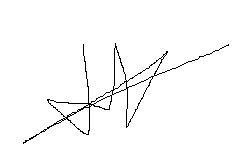
\includegraphics[width=0.4\textwidth]{imagenes/firma.png}\\[0.5cm]

\noindent Fdo: Juan del Río Gómez


\vspace{2cm}

\begin{flushright}
Granada a 1 de septiembre de 2023 .
\end{flushright}


\chapter*{}
\thispagestyle{empty}

\noindent\rule[-1ex]{\textwidth}{2pt}\\[4.5ex]

D. \textbf{Oresti Baños Legrán(tutor1)}, Profesor del Área de Ingeniería de Sistemas y Automática del Departamento de Ingeniería de Computadores, Automática y Robótica de la Universidad de Granada.

\vspace{0.5cm}

D. \textbf{Miguel Damas Hermoso (tutor2)}, Profesor del Área de de Ingeniería de Sistemas y Automática del Departamento de Ingeniería de Computadores, Automática y Robótica de la Universidad de Granada.


\vspace{0.5cm}

\textbf{Informan:}

\vspace{0.5cm}

Que el presente trabajo, titulado \textit{\textbf{POSTCOVID-AI TelegramBot}},
ha sido realizado bajo su supervisión por \textbf{Juan del Río Gómez (alumno)}, y autorizamos la defensa de dicho trabajo ante el tribunal
que corresponda.

\vspace{0.5cm}

Y para que conste, expiden y firman el presente informe en Granada a 1 de Septiembre de 2023.

\vspace{1cm}

\textbf{Los directores:}

\vspace{5cm}

\noindent \textbf{Oresti Baños Legrán (tutor1) \ \ \ \ \ Miguel Damas Hermoso(tutor2)}

\chapter*{Agradecimientos}
\thispagestyle{empty}

       \vspace{1cm}

En primer lugar quisiera agradecer a mi familia, sin su ayuda hoy no estaría donde estoy.

A todos mis compañeros de carrera y amigos, siempre dispuestos y atentos a ayudarme a resolver problemas del día a día.

Y a todos los profesores que me han aportado experiencias positivas gracias a su enseñanza durante el transcurso de esta bonita etapa. 
    



%\frontmatter
\tableofcontents
\listoffigures
%\listoftables
%
\setlength{\parskip}{5pt}

\chapter{Introducción}

En la historia de la humanidad surgen momentos y etapas que transcienden lo cotidiano y se convierten en hitos definitorios de una era. Uno de estos hitos que han marcado una etapa adversa en la historia moderna ha sido la pandemia de COVID-19, cuyos síntomas han afectado en cada rincón del planeta y han sacudido los cimientos de nuestra existencia de manera profunda. 

Cada uno de nosotros en cierta medida, hemos experimentado un crisol de emociones y desafíos que invitan a la introspección y la búsqueda de significado a la adversidad. La soledad ocasionada por el confinamiento y alejamiento de nuestras personas queridas, la ansiedad, la depresión y el estrés se volvieron parte del día a día de muchas personas.

En medio de todo este revuelo, la mente humana, enrevesada, reaccionó planteándose algunas preguntas existenciales ¿Qué valores importan en tiempos de crisis? ¿Cómo podemos encontrar la fortaleza para luchar contra la incertidumbre? 

Esto ha provocado que la población haya tenido que experimentar un periodo de adaptación a esta nueva normalidad. Ha habido un gran cambio en el desarrollo del cerebro de la población juvenil provocado por el confinamiento, la vulnerabilidad psicosocial y aumento a la exposición a las redes sociales. Como vemos en la \textit{\hyperref[fig:impacto]{figura 1.1}} esto afecta a las habilidades socioemocionales, generando conductas de agresividad, falta de empatía, ansiedad, síntomas depresivos, dificultades para la resolución de conflictos\textit{(\cite{psychiatry2020})}. 

Y no solo en este sentido, ya que el bienestar se refiere a un estado general de satisfacción y equilibrio en la vida y se compone de varios aspectos, como la salud física, la salud mental, la calidad de vida y el sentido de propósito y conexión con los demás\textit{(\cite{bienestar})}. Por lo que debemos tener en cuenta que el bienestar no es un aspecto individual, sino que se encuentra asociado al entorno en el que vivimos y que nos ayuda a hacer frente a los factores estresantes de la vida, a aprender y trabajar bien, y a contribuir a nuestra comunidad.

En definitiva, la importancia del bienestar se ha vuelto crucial, ya que la pandemia ha afectado significativamente a la calidad de vida de las personas. Es esencial abordar el bienestar como una cuestión de interés público y trabajar juntos para construir una sociedad más saludable y equitativa. 

Este proyecto nace en este contexto, con el objetivo de contribuir a la mejora de la salud mental a través de la tecnología, ofreciendo un medio cómodo para la recogida de datos que permita la detección de tendencias relacionadas con problemas de salud mental y nos ayude a combatir este problema.

\begin{figure}[!ht]
    \centering
    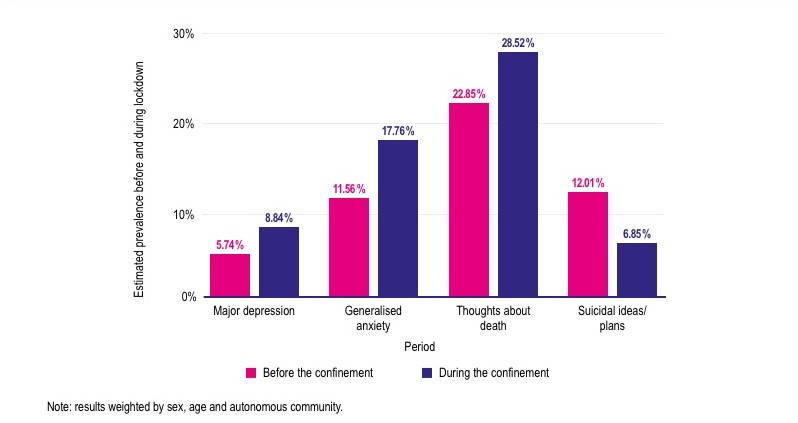
\includegraphics[width=1\textwidth]{imagenes/graficaCovid.jpg}
    \caption{ Comparación de personas con problemas mentales antes y durante la pandemia por\textit{(\cite{impactocovid})}}
    \label{fig:impacto}
\end{figure}


\section{Motivación}

La nueva normalidad socioeconómica tras el brote de COVID-19 plantea desafíos sin precedentes tanto para los gobiernos como para los ciudadanos. Desde el inicio de la pandemia los gobiernos han tenido acceso a diversos datos económicos, pero la información precisa sobre cómo la nueva normalidad y las políticas específicas influyen en la conducta individual y grupal y, en consecuencia, en el bienestar de la sociedad, es escasa, indirecta y abierta a la interpretación. Como argumenta \textit{(\cite{medicion2009})} son necesarios datos que proporcionen un indicador cuantitativo confiable de cómo las diferentes medidas y su impacto en el contexto económico, social y conductual afectan el bienestar general de la población.\vspace{0.3cm}

Gracias al uso masivo de teléfonos inteligentes podemos recoger datos ubicuos, continuos y anónimos de la población, así como datos emocionales, sociales, conductuales y relativos al bienestar.\vspace{0.3cm}

En este contexto, la creación de un agente conversacional en \href{https://telegram.com.es/}{\textit{(Telegram)}} se nos presenta como una ingeniosa solución para esta recolección de datos. La motivación de este proyecto radica en la importancia de poder brindar al usuario un espacio confidencial y seguro a través de conversaciones interactivas y personalizadas para que las personas puedan expresar sus emociones sin ningún tipo de pensamiento crítico.
Además Telegram consta de un diseño atractivo permitiendo la integración de cuestionarios, encuestas, enlaces, lo que facilita el acceso a recursos de apoyo.\vspace{0.3cm}

Toda esta información recogida puede ser muy útil para investigadores y profesionales del sector, ya que proporcionan una visión más precisa de las necesidades y desafíos a los que se enfrentan los ciudadanos. 


\begin{quote}
    \textit{"De vez en cuando, una nueva tecnología, un antiguo problema y una gran idea se convierten en una innovación"} \\ 
    -- Dean Kamen. Creador del Segway y el iBOT.
\end{quote}

\section{Objetivos}

Este proyecto tiene como objetivo el desarrollo de un chatbot con el que recabar información personal sobre aspectos claves en el bienestar de las personas, de forma que nos permita clasificarla y estructurarla para generar un análisis. 

Para lograr este objetivo general se plantean los siguientes objetivos específicos:

\begin{itemize}
    \item Creación del chatbot para la recogida de datos relacionados con el bienestar.
    \item Creación de una interfaz para comunicarnos con el chatbot.
    \item Implementación de la lógica interna propia del chatbot para adaptarse al contexto que estemos hablando y dar una respuesta digna.
    \item Desarrollo de una aplicación web que nos permita interactuar con el chatbot y las preguntas a realizar.
    \item Almacenamiento de las preguntas y respuestas en la base de datos de forma automática.
\end{itemize}

\section{Estructura}

En este primer capítulo hemos visto una introducción del proyecto, comentando la motivación del mismo y los objetivos a cumplir a lo largo de este desarrollo. En el segundo capítulo, nos pondremos un poco más en contexto y veremos ejemplos de chatbots en la actualidad relacionados con nuestro tema e intentaremos entender como funcionan, como nos ayudan y forman parte de nuestro día a día.

En el tercer y cuarto capítulo hablaremos sobre la planificación y etapas seguidas en el ciclo de vida del proyecto. Indagaremos en las tecnologías usadas, los requerimientos necesarios de nuestro trabajo, exponiendo las funcionalidades de todas las partes implicadas, problemas a abordar y como satisfacerlos. Seguidamente en los capítulos posteriores encontraremos toda la información necesaria para entender el desarrollo y la implementación del proyecto, para finalizar con la puesta a punto, conclusiones, aspectos a mejorar y una guía de uso para el usuario. 

\chapter{Estado del arte}

\section{Chatbots}

Un chatbot o agente conversacional es un programa inteligente que mediante lenguaje escrito u oral pueden interactuar con los usuarios a través de una conversación de lenguaje natural. 

Los chatbots se han convertido en una forma cada vez más popular de que las empresas interactúen con sus clientes. Proporcionan una forma cómoda y eficaz de obtener respuestas a las consultas de los clientes, ayudarles a realizar compras e incluso ofrecerles recomendaciones personalizadas. Como resultado, cada vez más empresas están implementando chatbots en sus operaciones de atención al cliente. En este artículo, analizaremos las diversas formas en que las empresas están aprovechando la tecnología de chatbot para mejorar su experiencia de servicio al cliente y cómo se pueden utilizar también en otras áreas de negocio.

\begin{figure}[!ht]
    \centering
    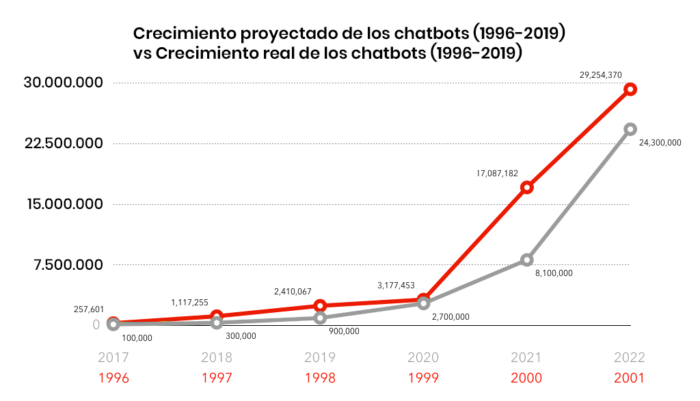
\includegraphics[width=1\textwidth, height=5.5cm]{imagenes/uso_chatbots.png}
    \caption{ Crecimiento del uso de chatbots en los últimos años }
    \label{fig:enter-label}
\end{figure}

\subsection{Tipos de chatbots}

Un chatbot funciona de un par de maneras: con directrices establecidas y mediante aprendizaje automático (ML).{\vspace{0.3cm}

\textit{\textbf{Set Guidelines Chatbots}}: Un chatbot que funciona con un conjunto de directrices establecidas está limitado en su conversación. Sólo puede responder a un número determinado de peticiones y vocabulario y es tan inteligente como su código de programación. Un ejemplo de bot limitado es un bot bancario automatizado que hace algunas preguntas a la persona que llama para entender lo que quiere hacer.{\vspace{0.3cm}


\textit{\textbf{Machine Learning Chatbots}}: Un chatbot que funciona mediante aprendizaje automático tiene una red neuronal artificial inspirada en los nodos neuronales del cerebro humano. El bot está programado para autoaprender a medida que se le presentan nuevos diálogos y palabras. En efecto, a medida que un chatbot recibe nuevos diálogos de voz o textuales, aumenta el número de consultas a las que puede responder y la precisión de cada respuesta que da.


Los chatbots se utilizan en diferentes sectores y se crean con diferentes fines. Hay bots de venta al por menor diseñados para recoger y encargar la compra, bots meteorológicos que dan la previsión del tiempo del día o de la semana, y bots simplemente amistosos que simplemente hablan con la gente que necesita un amigo.

\subsection{Canales de comunicación}

Los canales de comunicación desempeñan un papel importante a la hora de ayudar a las marcas y a los clientes a conectarse entre sí para diversas formas de compromiso e interacciones. La elección del canal adecuado es vital para que nuestro chatbot proporcione una experiencia efectiva y eficiente en los usuarios. Algunos de los más usados son:\vspace{0.3cm}

\textbf{Sitio Web y App móvil}: Uno de los canales más populares es en el sitio web de la empresa o en algunos casos en la App que dispongan. El chatbot puede responder preguntas frecuentes de los clientes y proporcionar asistencia en tiempo real.\vspace{0.3cm}

\textbf{Facebook}: Otra forma es integrándolo el chatbot en una página de Facebook. A través de Facebook Messenger los clientes pueden recibir respuestas automáticas al momento. Además Facebook brinda la oportunidad de integrar el chatbot en tu página para que responda comentarios de tu muro de forma automática.\vspace{0.3cm}

\textbf{WhatsApp}: Creando una cuenta en WhatsApp Business API, el bot puede responder instantáneamente al usuario y segmentar las conversaciones. \vspace{0.3cm}

\textbf{Telegram}: Surge como alternativa a la preeminente WhatsApp. Desde entonces, ha sido percibida como una aplicación más segura que su rival, debido a sus políticas de encriptación. Además permite la creación de bots en grupos de hasta 100.000 personas.\vspace{0.3cm}

\textbf{Google My Business}: Permite chatear con cualquier persona que encuentre tu negocio a través de Google.




\subsection{Ventajas y desventajas de usar chatbots}
{\vspace{0.5cm}

\begin{table}[!ht]
\begin{center}
\begin{tabular}{| p{6cm} | p{7cm} |}
\hline
\rowcolor{blueice}
\textbf{Ventajas} & \textbf{Desventajas} \\
 \hline
- Menor coste que trabajadores humanos & - Puede no entender las consultas de los usuarios \\
- Online 24/7 & - Carece de emoción y no es personalizable \\
- Puede usarse como herramienta de ventas, marketing y recopilación de información & - Necesitan mantenimiento constante \\ \hline
\end{tabular}
\end{center}
\end{table}



\section{Trabajos previos}

Los chatbots se pueden aplicar a diferentes áreas. En el caso de salud mental podemos ver bots conversacionales que actúan como psicólogos para las personas como por ejemplo \textit{(\cite{vivibot2019})}. Proponen un bot conversacional para proporcionar habilidades de psicología positiva y promover el bienestar entre los jóvenes después del tratamiento del cáncer. Reclutaron a adultos jóvenes en los 5 años siguientes a la finalización de un tratamiento activo contra el cáncer a una prueba de 4 semanas para probar la efectividad del bot. Este incluía 4 semanas de habilidades de psicología positiva, valoraciones diarias de emociones, vídeos y otros materiales. Los análisis examinaron la participación del chatbot y los comentarios abiertos sobre la simpatía y la utilidad percibida y compararon los grupos experimental y de control con respecto a los síntomas de ansiedad y depresión y los cambios en las emociones positivas y negativas entre el inicio y las 4 semanas. Los participantes calificaron su experiencia de útil y recomendada. Los comentarios abiertos señalaron su naturaleza no crítica como una ventaja particular del chatbot.{\vspace{0.3cm}

Otro ejemplo de bot conversacional orientado a la salud es \textit{(\cite{21daystressdetox2021})} que plantea un agente virtual para ayudar a adolescentes a afrontar los cambios importantes en su vida, como terminar los estudios o la formación, iniciar una carrera profesional o entablar una relación íntima que pueden desencadenar o amplificar problemas de salud mental subyacentes, lo que a veces provoca un malestar psicológico o un funcionamiento inadaptado. {\vspace{0.3cm}

\textit{(\cite{moodfit2016})} es una aplicación que pretende ayudar a los consumidores a comprender y mejorar su estado de ánimo, aumentar su resiliencia y alcanzar objetivos. Utiliza principios cognitivo-conductuales (TCC) como el registro de pensamientos, la atención plena, la meditación y el diario de gratitud para tratar las fluctuaciones del estado de ánimo que pueden deberse a la depresión, el estrés y la ansiedad. Los consumidores pueden crear sus propios objetivos o elegir entre los predeterminados, como estado de ánimo, sueño, gratitud y nutrición. La pantalla de inicio muestra el porcentaje de objetivos que el consumidor ha alcanzado junto con cuántos días ha guardado su estado de ánimo de forma consecutiva. También hay recordatorios que ofrecen consejos para mejorar el estado de ánimo, así como una sección que hace un seguimiento del progreso del usuario con gráficos.


\section{Procesamiento del Lenguaje Natural (PLN)}

El procesamiento del lenguaje natural (PLN) es una rama de la Inteligencia Artificial (IA) que se ocupa de comprender y generar el lenguaje humano. Ayuda a las máquinas a entender el significado de palabras, frases y oraciones para generar resultados con sentido. La tecnología PLN se ha hecho cada vez más popular en los últimos años gracias a su capacidad para automatizar tareas mundanas como la extracción de datos, el resumen de textos, el análisis de sentimientos, etc.{\vspace{0.3cm}


Los asistentes virtuales o chatbots son una de las utilidades más conocidas de la PLN, pero no son la única. Además, es importante entender que el PLN no dota de inteligencia a un chatbot, sólo le da la capacidad de procesar y generar lenguaje humano. En caso de querer dotar de inteligencia a un asistente virtual, habría que utilizar sistemas como reglas o redes neuronales.{\vspace{0.3cm}


La PNL puede dividirse en dos tipos principales: basada en reglas y estadística. La PNL basada en reglas utiliza reglas predefinidas para analizar los datos de entrada, mientras que la PNL estadística utiliza técnicas de aprendizaje automático para aprender de las muestras de datos. Ambos enfoques tienen sus ventajas e inconvenientes en función de la aplicación para la que se utilicen.\vspace{1cm}


\subsection{Beneficios del PLN}

El procesamiento del lenguaje natural (PLN) es un avance de vanguardia por varias razones.{\vspace{0.3cm}

- Permite a los no expertos en la materia encontrar respuestas a sus preguntas.{\vspace{0.1cm}

- Analizar datos de fuentes estructuradas y no estructuradas.{\vspace{0.1cm}

- Identificar las causas profundas de los problemas de su empresa.{\vspace{0.1cm}

- Descubra a sus clientes más rentables y comprenda las razones que hay detrás de ello.{\vspace{0.1cm}

- Identificar y abordar las reclamaciones y comportamientos fraudulentos.{\vspace{0.1cm}

- Comprender varios idiomas, dialectos, jerga y argot.{\vspace{0.1cm}

- Identificar patrones en la comunicación con los clientes y reducir sus quejas.{\vspace{0.1cm}

- Analizar y evaluar la oferta de productos de sus competidores.{\vspace{0.1cm}


\chapter{Planificación y presupuesto}

En el mundo de la gestión de proyectos, nos encontramos con varias etapas que guían el rumbo y éxito de cualquier iniciativa. Es un ciclo continuo con diversas fases interconectadas conocidas como el 'Ciclo de vida de un proyecto'. 

En esta sección haremos un recorrido comentando el ciclo de vida del proyecto, desglosando la planificación, y haciendo una estimación sobre el coste que supone el desarrollo del mismo.\vspace{0.3cm}

\section{Planificación}

La planificación de un proyecto tiene como objetivo su realización en las condiciones ideales y asegurando los mejores resultados. Este ciclo de vida es un marco conceptual que divide la evolución de un proyecto en etapas secuenciales, cada una con sus diferentes objetivos. Para el desarrollo de este proyecto se han seguido las siguientes etapas. 

\begin{itemize}
    \item \textbf{Estudio} de distintos tipos de chatbots y trabajos similares que nos servirán como ejemplo a la hora de definir la funcionalidad del proyecto. Realización de cursos y estudio de la documentación de las tecnologías que vamos a usar.
    \item \textbf{Documentación} de la memoria realizada concurrentemente en todas las etapas del proyecto. 
    \item \textbf{Análisis} del proyecto, identificando los requisitos, entidades y componentes, así como la forma de interactuar entre sí. 
    \item \textbf{Diseño} de la base de datos, generación de mockups para las interfaces de usuario y arquitectura. 
    \item \textbf{Implementación} del software teniendo en cuenta todo los aspectos estudiados en las etapas previas.
    \item \textbf{Evaluación y corrección de errores} realizando pruebas constantes y exponiendo todos los casos de uso posibles para la detección de errores y su correcto arreglo. 
    \vspace{0.3cm}
    \item \textbf{Despliegue} del proyecto en un contenedor software y subida a github para que su instalación sea lo más sencilla posible. 
    
\end{itemize}\vspace{0.5cm}

\begin{figure}[!ht]
    \centering
    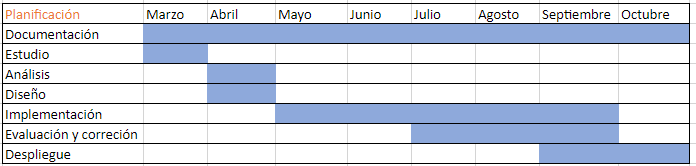
\includegraphics[width=1\textwidth]{imagenes/plan.png}
    \caption{ Planificación temporal }
    \label{fig:planificacion}
\end{figure}
\vspace{1cm}

\section{Presupuesto}

\subsection{Requerimientos software}

Todos los recursos software y tecnologías utilizadas en el proyecto son gratuitos. Partiendo desde el IDE utilizado en mi caso Visual Studio Code, como los framework Django y Foundation, Docker, todas las librerías, e incluso la conexión a la API de Telegram. Además se encuentra subido en un repositorio público de github, que nos ayuda a realizar copias y controlar versiones. 

El único gasto en recursos sería el despliegue del proyecto en un servidor. Si quisieramos migrarlo a la nube en Amazon Web Services un precio medio teniendo en cuenta varios factores como el tamaño de la instancia EC2, capacidad de almacenamiento de la base de datos y transferencia de datos nos costaría aproximadamente entre 40 y 70 euros por mes según \textit{(\cite{aws2022})}, que es lo que cuesta la arquitectura más básica. 

Cabe destacar que Amazon cobra toda la transferencia de datos que sucede por fuera de su misma red, es decir, cada dato que nosotros queramos mover dentro y fuera de AWS nos costará.


\subsection{Recursos humanos}


Teniendo en cuenta que este proyecto es desarrollado única y exclusivamente por mí, el coste de recursos humanos, contando las horas efectivas trabajadas en el proyecto por el autor y estableciendo un salario base de un programador de unos 14,62€ la hora según  \textit{(\cite{salario2022})} sería el siguiente:\vspace{0.5cm}


\begin{table}[!ht]
    \begin{center} 
    \begin{tabular}{| c | c | c |}
    \hline
    \rowcolor{blueice}
    Actividad & Horas & Coste  \\ \hline
    Análisis y diseño & 25h & 365€\\
    Implementación & 200h &  2924€\\
    Evaluación y corrección & 80h & 1169€ \\ \
    Despliegue & 10h & 146€ \\ 
    Documentación & 50h & 731€ \\ \hline
    \rowcolor{gray30}
    Total & 365h & 5336€ \\ \hline
    \end{tabular}
    \caption{Tabla presupuesto}
    \label{tab:presupuesto}
    \end{center}
\end{table}




\chapter{Análisis}

\section{Arquitectura}
El objetivo del chatbot es conseguir información estructurada a partir de las experiencias y emociones de los usuarios. Con este objetivo se ha desarrollado un proyecto que consta de dos componentes principales: una aplicación web y un chatbot en Telegram. La aplicación web actúa como panel de control para que el administrador tenga acceso a la gestión de preguntas, así como consultar las respuestas de los usuarios. 

Para asegurar la eficacia, se hace uso de una base de datos tipo PostgreSQL que almacena tanto las preguntas como las repsuestas lo que permite un fácil acceso a esta información. Gracias a esto se consigue una solución integral que combina la facilidad de uso del chatbot en Telegram con la capacidad de gestión y análisis dada por la aplicación web. \vspace{7cm}


\begin{figure}[!ht]
    \centering
    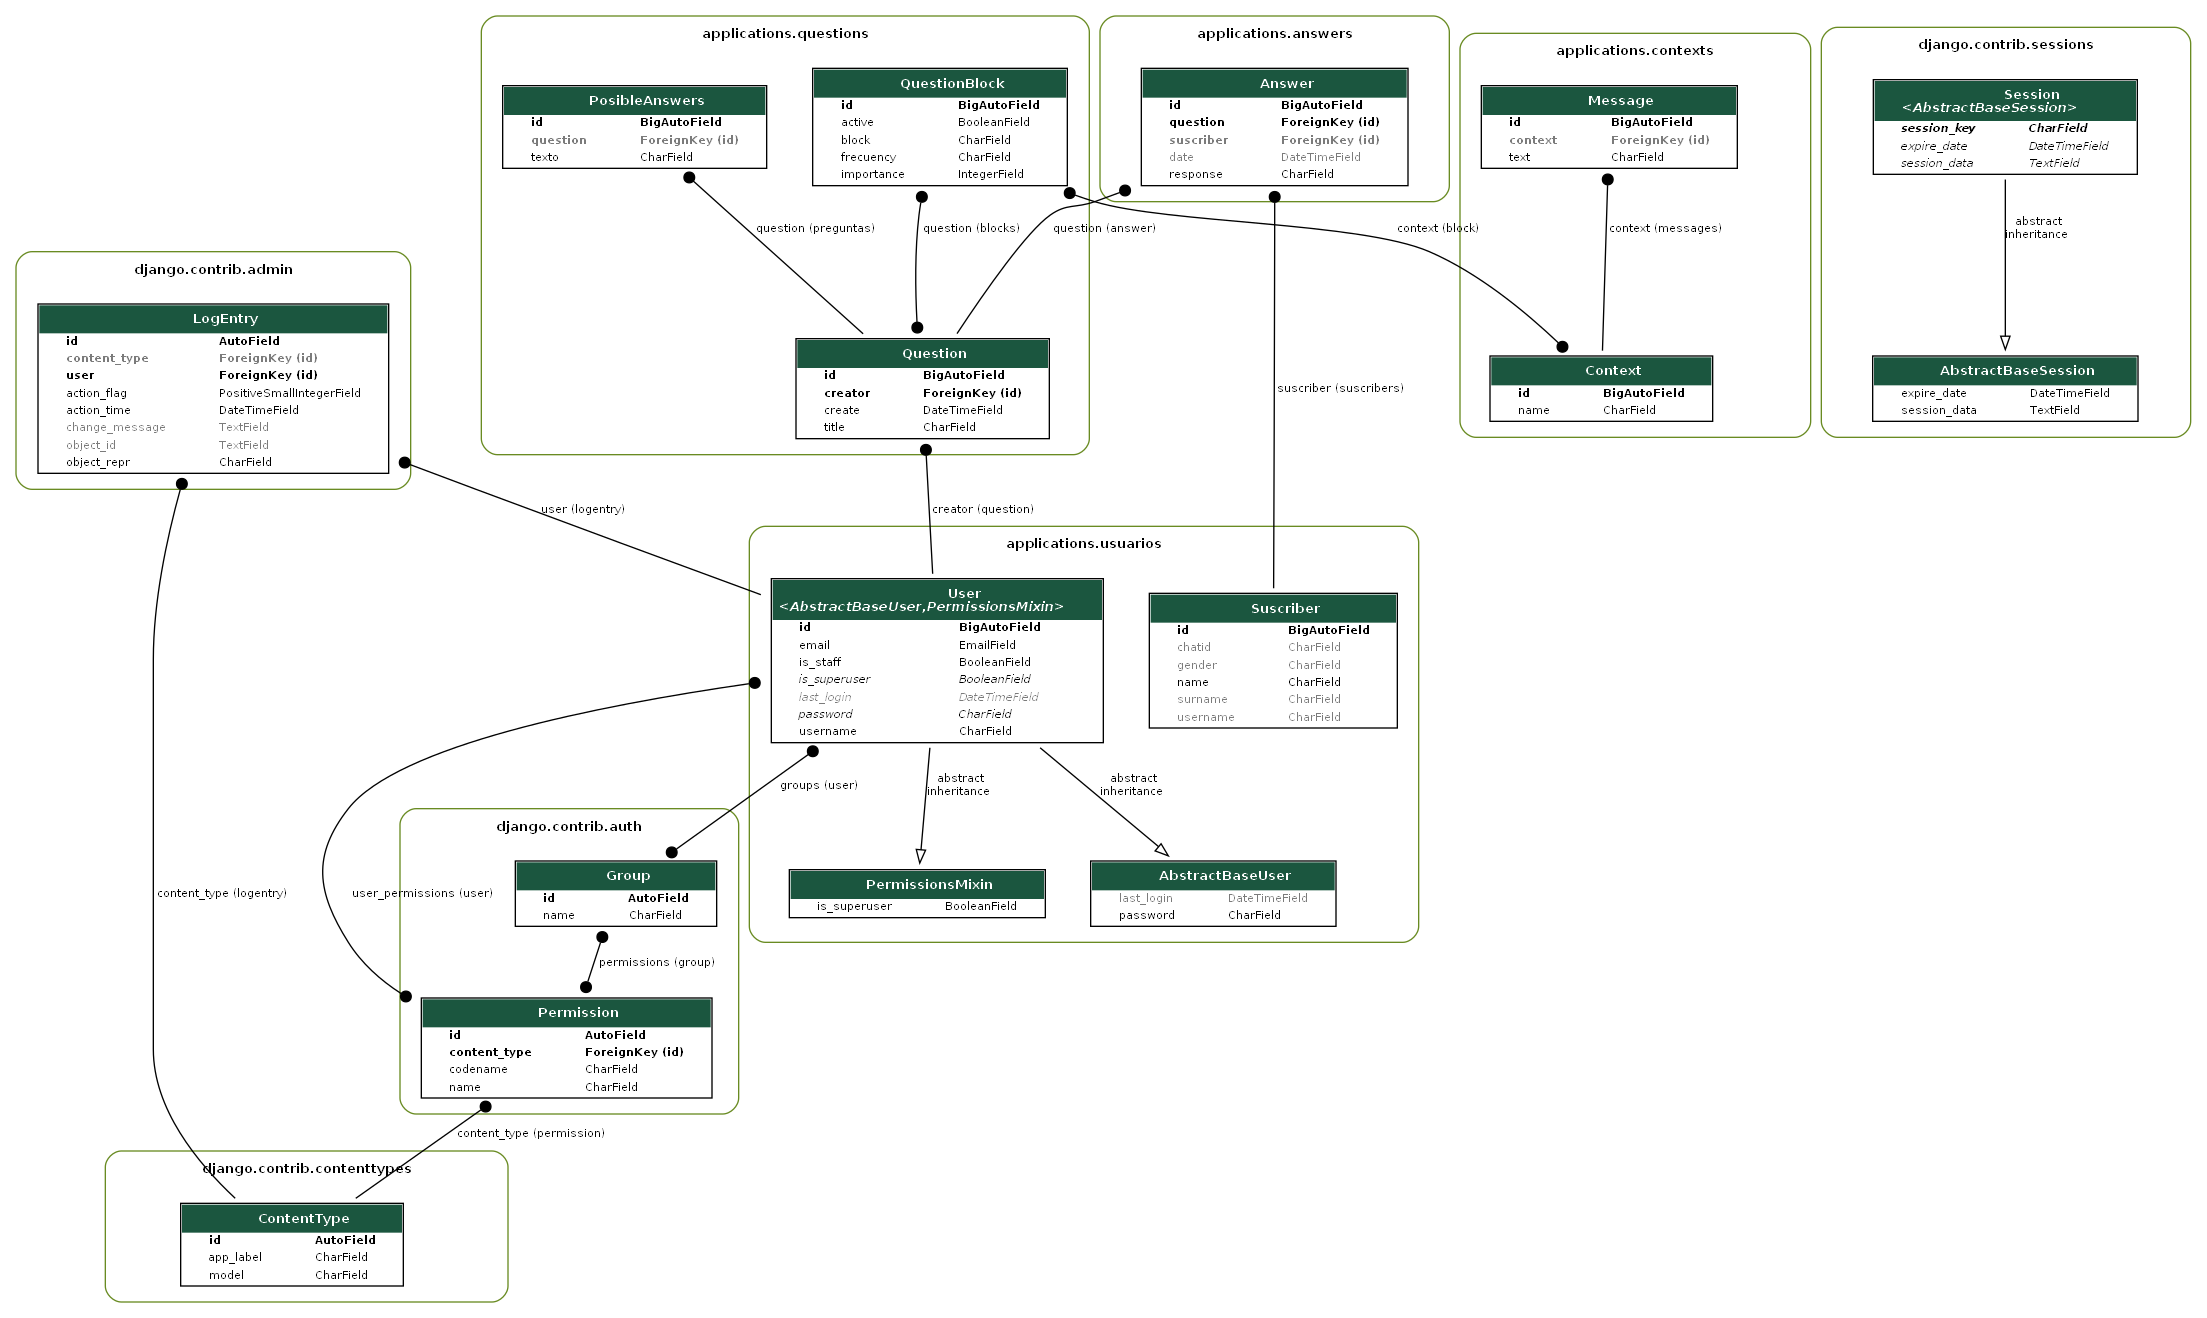
\includegraphics[width=1\textwidth, height=15cm]{imagenes/myapp_models.png}
    \caption{ Diagrama de clases }
    \label{fig:enter-label}
\end{figure}


Esta base de datos consta de cinco entidades principales:
\begin{itemize}
\item \textbf{Peguntas}: Contiene la información de todas las preguntas almacenadas. Esta se divide en dos: Pregunta y Posibles respuestas. Dentro de la primera especificaría el título de la pregunta junto con otros campos como la fecha o usuario de creación y la segunda contiene las respuestas a esa pregunta. 
\item \textbf{Bloques de Preguntas}: Las preguntas se almacenan en bloques. Cada bloque puede tener las preguntas que desee, además de un atributo booleano que indicará que ese bloque de preguntas se encuentra activo. Los bloques también tienen asociado un contexto. 
\item \textbf{Contextos}: Dentro de los contextos se guardan los mensajes a mostrar por el bot cuando se hable de un tema concreto. Si un bloque tiene asociado un contexto, en el momento que se realice el cuestionario asociado a ese bloque de preguntas el bot mostrará cualquiera de los mensajes de ese contexto de forma aleatoria. De esta forma nos aseguramos la interactividad y que la experiencia sea diferente para cada usuario.
\item \textbf{Usuarios}: Guarda los agentes registrados en nuestro sistema. Se divide en dos tipos: los administradores que tienen acceso al panel de control y los usuarios comúnes que son los que interactúan con el bot.
\item \textbf{Respuestas}: Contiene las respuestas de los usuarios a las preguntas. Solo se almacenan las respuestas posibles de cada pregunta para así confirmar que la información sea correcta.
\end{itemize}

La parte del chatbot está formada por tres módulos. Un primer módulo de bienvenida y registro, donde el bot se presenta con el usuario y lo registra en nuestra base de datos. Un segundo módulo que actúa como agente conversacional y un tercer módulo que representa el cuestionario de preguntas. Posteriormente los analizaremos con más detalle.

Esta arquitectura permite creación de cuestionarios interactivos, almacenamiento de datos y análisis de respuestas de forma confidencial para su posterior evaluación.

\begin{figure}[h]
    \centering
    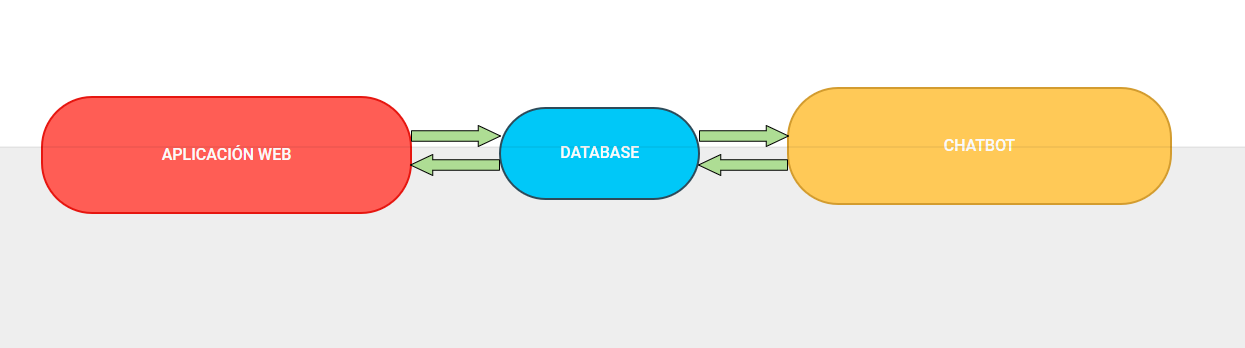
\includegraphics[width=1\textwidth]{imagenes/arquitecture.png}
    \caption{\textit{POSTCOVID-AI TELEGRAMBOT} arquitectura}
    \label{fig:enter-label}
\end{figure}

\section{Implementación}
Para el desarrollo usaremos herramientas de Front-End, que nos ayudarán a dar cuerpo a nuestro sitio web y herramientas de Back-End para el control y lógica tanto de la web como del bot. Las tecnologías utilizadas para la implementación del proyecto son las siguientes:

\begin{itemize}
\item \textit{\textbf{Python}} como lenguaje principal del bot y de la web.
\item \textit{\textbf{Django}} es un framework de aplicaciones web gratuito y de código abierto (open source) escrito en Python para el desarrollo de nuestra web.
\item \textit{\textbf{Telegram}} como plataforma para alojar el chatbot
\item \textit{\textbf{Python-telegram-bot}} es una librería de Python para la creación de nuestro bot que nos permite conectarnos a la API de Telegram.
\item \textit{\textbf{PostgreSQL}} es un sistema de gestión de base de datos relacional orientado a objetos.
\item \textit{\textbf{Psycopg2}} para adaptar la base de datos a Python.
\item \textit{\textbf{HTML5}} lenguaje para la elaboración de páginas web.
\item \textit{\textbf{CSS3}} como lenguaje de diseño gráfico para crear la presentación de nuestra página.
\item \textit{\textbf{Javascript}} para dar dinamismo a nuestra web y ayudar en la experiencia del usuario.
\item \textit{\textbf{Foundation}} como framework de ayuda a la hora de crear la interfaz de usuario.
\item \textit{\textbf{Docker}} para automatizar el despliegue de la aplicación dentro de un contenedor software.
\item \textit{\textbf{Github}} como tecnología que nos ayuda a realizar copias del proyecto y controlar versiones.
\end{itemize}


\section{Funcionamiento}
Antes de empezar con el desarrollo de nuestro proyecto, debemos definir la funcionalidad del mismo explicando detalladamente como sería el comportamiento de cada una de las partes implicadas.

\begin{itemize}
\item \textbf{Web}: Creación de una interfaz con la que poder interaccionar con las preguntas del bot y mensajes a mostar.
\begin{itemize}
\item Implementación de un login y un registro para que solo los usuarios registrados puedan acceder al panel de control.
\item Panel de control, primera vista del usuario que funciona como guía para las operaciones a realizar.
\item Apartado de preguntas, bloques, contextos, preguntas e información y gestión de usuarios.
\item Vistas de detalle y operaciones de modificación y borrado de cada uno de los apartados anteriores.
\item Autenticación y permisos en la realización de operaciones solo para usuarios específicos.
\item Descarga de las respuestas proporcionadas por los usuarios en formato CSV.

\end{itemize}
\item \textbf{Chatbot}: Creación de un chatbot en línea que realice un cuestionario de preguntas y a su vez una lógica interna que permita una interacción con el usuario.
\begin{itemize}
\item Mensaje de bienvenida al usuario cuando entre en el chat del bot.
\item Almacenamiento del usuario como un nuevo integrante de nuestro sistema si ningún tipo de cuestionario gracias a las funciones especificas de Telegram que permiten la obtención de los datos del usuario que se encuentra activo en el chat.
\item Entorno de interacción por parte del bot con el usuario para poder tener una conversación lo más humana posible mediante el análisis de ciertas palabras e ideas previamente establecidas.
\item Cuestionario de preguntas que se encuentran activas para cada usuario en un momento concreto. Estas preguntas varían dependiendo de los bloques que el administrador tenga activos y la frecuencia de cada uno de ellos.
\item Recolección y almacenamiento de las respuestas proporcionadas en la base de datos de forma automática.
\item Lógica para identificar cada vez que el usuario cuente con preguntas activas.
\item Creación de un aviso diario al usuario cuando haya preguntas sin responder.
\end{itemize}
\end{itemize}

%
\chapter{Chatbot}

El objetivo del bot es la recaudación de datos de usuarios mediante el uso de un agente conversacional como alternativa al tradicional cuestionario de preguntas. Para que al usuario le sea atractivo responder este tipo de cuestionarios que usualmente suelen ser un poco monótonos, he implementado una parte de interacción básica. Leyendo varias fuentes y opiniones de usuarios acerca de su experiencia con chatbots, 
 en \textit{(\cite{wellbeingchabot})} llegan a la conclusión de que a las personas entrevistadas les es mucho mas fácil poder abrirse y contestar preguntas acerca de su salud con un chatbot con el que pudieran conversar sabiendo que no hay lugar a ninguna crítica ni prejuicio por su parte, además de ser una experiencia calificada como más entretenida y divertida que realizar un cuestionario. Partiendo de esta base y con esa idea se ha desarrollado este proyecto. 

El agente conversacional se encuentra formado por 3 módulos diferenciados: Módulo de bienvenida y registro de usuario, módulo conversacional y cuestionario

\section{Módulo de bienvenida y registro}

La libreria \textit{python-telegram-bot} es la herramienta con la que vamos a interactuar con la API de Telegram. La librería emerge como una herramienta indispensable en este ámbito, proporcionando a los desarrolladores un marco completo para construir, desplegar y gestionar bots de Telegram sin esfuerzo.

Esta nos va a permitir diferentes posibilidades a la hora de crear nuestro bot como son la gestión de actualizaciones para controlar diferentes tipos de entradas de manera eficiente, envío de mensajes de texto y contenido multimendia, teclados y botones, comandos personalizados, respuestas interactivas, middleware y filtros. Todo lo relacionado a la descripción de estas operaciones se encuentra especificado en la documentación oficial \textit{(\cite{pythontelegrambot})}.

Este primer módulo tiene como objetivo la presentación de nuestro bot con el usuario y su registro en nuestra base de datos. 

Este módulo contiene una función que es la primera que se ejecuta cuando cualquier persona empieza una conversación. Se activa con el comando \textit{/start} que se envía mecánicamente y es el único comando necesario para la conversación. Cuando este evento se detecta se realiza una llamada a la función la cual muestra un mensaje de bienvenida al usuario presentando los temas a tratar. Gracias a la librería usada podemos obtener los datos que el usuario posea en su Telegram personal (como el nombre, nombre de usuario, apellidos, email, id).\vspace{0.3cm}

\begin{lstlisting}[language=Python]
    suscriber, created = Suscriber.objects.get_or_create(
        chatid = chat_id,
        name=name,
        surname=surname,
        username=username,
    )
\end{lstlisting}

 La función de Django \textit{get\_or\_create()} nos permite filtrar una serie de datos introducidos dentro de una tabla en la base de datos. En caso de que ningún registro coincida exactamente con todos los datos, crea una nueva instancia con los parámentros pasados. De esta forma se registran los usuarios. Para asegurarnos de la concurrencia de nuestro programa, he creado un atributo en usuario llamado chatid que almacena el id propio del chat. Esto se hace con la intención de no declarar variables globales dentro del código ya que si hubiera varias personas hablando al mismo tiempo habría problemas de concurrencia. Por eso cada consulta y cada mensaje es específico para cada uno intentando operar siempre desde la base de datos, lo que además influye positivamente en la eficiencia ya que las consultas y operaciones son más rápidas.


\begin{figure}[!ht]
    \centering
    
\includegraphics[width=0.8\textwidth, height=4cm]{imagenes/welcome.png}
    \caption{ Mensaje de bienvenida }
    \label{fig:welcome}
\end{figure}

La figura \textit{\hyperref[fig:welcome]{figura 5.1}} muestra como es el mensaje de presentación del bot. Nos pone en contexto y nos habla sobre su propósito. Finalmente nos hace una pregunta y dependiendo de la respuesta del usuario nos redigirá a un módulo u otro. 

\section{Módulo conversacional}

Este módulo es una etapa intermedia, que funciona como una especie de sala de espera a que el usuario cuente con cuestionarios a responder. Dentro de él, se puede tener una conversación de lo más común y simple con el bot, con un apartado que muestra preguntas frecuentes en caso de que el usuario tenga cualquier tipo de duda. 

El usuario puede entrar dentro de este módulo de diferentes maneras. Una de ellas es respondiendo de forma negativa en la pregunta anterior. Dentro de este módulo hay unas palabaras, frases o expresiones previamente definidas por las cuales el bot responde en función de lo que escribas. Cabe destacar que no se utiliza modelos de lenguaje como GPT (Generative Pre-Trained Transformer) para generar respuestas mas elaboradas. GPT es un modelo que utiliza algoritmos avanzados de procesamiento de lenguaje natural para generar respuestas a preguntas y comentarios de los usuarios en tiempo real \textit{(\cite{gpt2020})}. En nuestro caso esa no es la finalidad de nuestro bot, como ya se ha indicado el propósito principal es la recogida de datos, con la funcionalidad añadida de que el usuario pueda tener una conversación escueta con el bot para que esta recogida se realice de la forma más humanamente posible, pero esta quedando siempre en segundo plano. 

Este módulo se ejecuta de forma recursiva cada vez que el usuario escribe un mensaje en el chat. Funciona de la siguiente manera:\vspace{0.3cm}

\textbf{1. Recogida del mensaje: }Cuando el usuario manda cualquier tipo de mensaje el bot lo recibe como texto de entrada y lo almacena.\vspace{0.3cm}

\textbf{2. Procesamiento: }Este proceso implica limpiar y normalizar el texto introducido, convirtiéndolo a minúsculas y reduciendo las palabras a su forma base. \vspace{0.3cm}

\textbf{3. Análisis: }Conlleva la identificación del contexto del mensaje con el propósito de extraer información relevante o identificar intenciones. 

Esta identificación se hace dentro del archivo \textit{replyMessages.py} situado dentro de la carpeta /chatbot. En el podemos encontrar diferentes listas como estas.\vspace{1cm}

\begin{lstlisting}[language=Python]
#HELLO AND GOOD BYE
greetings = ['hola', 'hello', 'buenos dias', 'buenas tardes', 'buenas', 'saludos', 'hi', 'good']
farewell = ['adios', 'bye', 'good bye', 'hasta luego', 'nos vemos', 'hasta pronto', 'buenas noches', 'que tengas un buen dia', 'hasta la proxima','que vaya bien']

\end{lstlisting}

Este es un ejemplo de lista para establecer el contexto de saludo y despedida. Estas listas definen una serie de palabras y expresiones concretas que cualquier persona hispanohablante utilizaría si quisiera referirse o hablar sobre un tema. Si cualquier palabra dentro de la respuesta del usuario se encuentra contenida en esta lista el bot identifica la intención del mensaje y le asociará un contexto.\vspace{0.3cm}

\textbf{4. Generación de respuesta: }Una vez encontrado el contexto del mensaje debemos buscar una respuesta digna que se adecue al tema tratado. Para ello dentro de este mismo archivo mencionado encontramos varios diccionarios. Estos contienen las respuestas que el bot debe proporcionar para cada contexto. Por ejemplo:

\begin{lstlisting}[language=Python]
    'greetings':{
        '0': 'Hola!¿Puedo ayudarte en algo?',
        '1': 'Muy buenas!¿Necesitas ayuda?',
        '2': 'Hola!¿Como puedo asistirte hoy?'
    },
    'farewell':{
        '0': '¡Adios!.¡Que tengas un buen dia!',
        '1': 'Hasta luego!.¡Espero verte de nuevo pronto!',
        '2': 'Adios. !No dudes en volver!',
    },
\end{lstlisting}

Cuando declaramos el contexto de saludo como este ejemplo, vemos que hay una serie de mensajes. He intentado que haya un mínimo de unos tres mensajes por cada contexto para que la respuesta proporcionada por el bot no sea siempre igual e intentar que esta varie. \vspace{0.1cm}

A la hora de mostrarlo en el chat se hace con la función de debajo que envía el mensaje al usuario en concreto que lo ha escrito y selecciona una respuesta aleatoria dentro de las que el diccionario disponga.\vspace{0.3cm}

\begin{lstlisting}[language=Python]
context.bot.send_message(chat_id=user.id, text=messages['greetings'][str(random_var)])
\end{lstlisting}

Por último debemos tratar que pasaría si el bot no reconoce el mensaje del usuario, ya sea por hablar de un tema que el bot no tiene respuesta o por escribir mal una palabra o expresión. En este caso, en la etapa anterior de análisis el bot no podría clasificar la respuesta. Cuando esto sucede se muestra lo que vemos en la \textit{\hyperref[fig:no-entendido]{figura 5.2}}\vspace{1cm}

\begin{figure}[!ht]
    \centering
    
\includegraphics[width=1\textwidth]{imagenes/no_respuesta.png}
    \caption{ Mensaje no entendido }
    \label{fig:no-entendido}
\end{figure}\vspace{0.3cm}

El mensaje contiene botones con algunas preguntas frecuentes que puedan ser de interés al usuario (como información sobre el bot, su propósito, sitio web y contacto del proyecto a que pertenece).En la \textit{\hyperref[fig:faq]{figura 5.3}} se pueden ver los mensajes que se mostrarían si se pulsa cada uno de los botones:\vspace{0.3cm}

\begin{figure}[!ht]
    \centering
    
\includegraphics[width=1\textwidth]{imagenes/preguntas_frecuentes.png}
    \caption{ Preguntas Frecuentes }
    \label{fig:faq}
\end{figure}\vspace{0.3cm}

\subsection{Job pendiente del usuario}

\vspace{0.5cm}

Desde el primer momento que el usuario entra dentro de este módulo se crea un proceso recursivo dentro del mismo que se ejecuta cada 24 horas. Este proceso se inicia cada vez que el usuario cuente con preguntas pendientes por responder. Para comprobar esto, el bot cuenta con un método que recorre las respuestas del usuario y compara la fecha de cuando esa pregunta fue respondida con la fecha actual. Recordemos que los bloques tienen una frecuencia, hay algunos que deben hacerse todos los días y otros una vez por semana. Pues esta función comprueba si el resultado de la resta de esta fecha pasado a segundos es mayor que la frecuencia del bloque también en segundos, significa que ha pasado el tiempo de frecuencia de ese bloque por lo que se vuelve a encontrar activo en el sistema y el usuario contará con preguntas pendientes. 

Cuando este usuario tenga preguntas se inicializa lo que según la libreria de \textit{python-telegram-bot} se denomina como 'Job'. Este Job es un proceso que se ejecuta cada un tiempo determinado y que solo termina cuando sucede un evento concreto. 

\begin{lstlisting}[language=Python]
    def create_job(self, context):
        #Create a user's job
        context.job_queue.run_repeating(callback=self.job, interval=86400, first=0, context=self.suscriber.chatid, name=self.suscriber.chatid)
\end{lstlisting}

Esta es una forma de crear el Job y como vemos este se ejecuta cada 24 horas y básicamente lo que hace es mostrar el mensaje mostrado en la \textit{\hyperref[fig:pending]{figura 5.4}} al usuario para avisarle de que tiene preguntas activas (si se cumple la condición de que las tenga) y puede pasar a responderlas.

\begin{figure}[!ht]
    \centering
    
\includegraphics[width=1\textwidth]{imagenes/mensaje_preguntasactivas.png}
    \caption{ Mensaje preguntas pendientes }
    \label{fig:pending}
\end{figure}

Este proceso solo termina cuando el usuario empieza a responder el cuestionario de preguntas. Si no lo hace, cada 24 horas el bot enviará el mensaje de nuevo. 

\section{Módulo cuestionario}


Pasamos ahora al último módulo y más importante de nuestro bot. Este módulo sigue el ejemplo de un cuestionario de preguntas clásico en el que el bot va haciendo una serie de preguntas y se debe responder con una de las opciones posibles conforme al criterio de cada uno. 

Para entrar, el bot ya sea al principio o cuando contemos con preguntas pendientes nos hará la pregunta de si queremos comenzar el cuestionario. Solo entraremos en él cuando respondamos de forma afirmativa a esta pregunta. 

Una vez estemos dentro, el bot nos explicará de forma escueta como funciona y eligirá la primera pregunta. He aquí cuando entra en juego una de las funciones principales \textit{chooseQuestion(user)}.

Esta función lo que hace es recorrer los bloques de preguntas que se encuentra activos en el sistema ordenándolos por importancia. Comprueba las preguntas una a una dentro de cada bloque filtrando las respuestas para cada usuario y comprobando si ha sido respondida. En este punto tenemos dos posibilidades. Que el usuario sea nuevo y no ha realizado ningún cuestionario, por lo que la primera pregunta que compruebe será la devuelta ya que no hay ningún registro de respuestas por su parte. Y en caso contrario, que el usuario ya haya realizado varios cuestionarios. En este supuesto, se resolvería de la misma forma que el Job entiende cuando un usuario cuenta con preguntas pendientes, es decir, comparando las fechas de las respuestas con la fecha actual, restándola y si es mayor a la frecuencia del bloque, significa que esa pregunta se encuentra pendiente, si no pasaría a la siguiente. Además el método identifica la primera pregunta perteneciente a cada bloque, para que cuando esta se haga muestre cualquiera de los mensajes asociados al contexto de ese bloque de preguntas.

Para el cuestionario, se ejecuta recursivamente la función \textit{handleanswer(update, context)} que es la encargada de realizar las preguntas, separándolas por bloques, mostrar los mensajes asociados a los contextos y recoger las respuestas como lo vemos en la \textit{\hyperref[fig:cuestionario]{figura 5.5}}. Solo termina cuando el usuario no cuente con preguntas pendientes. En cada iteracción hace una llamada a la función anterior \textit{chooseQuestion(user)}, eligiendo de forma dinámica la siguiente pregunta a realizar. 

\begin{figure}[!ht]
    \centering
    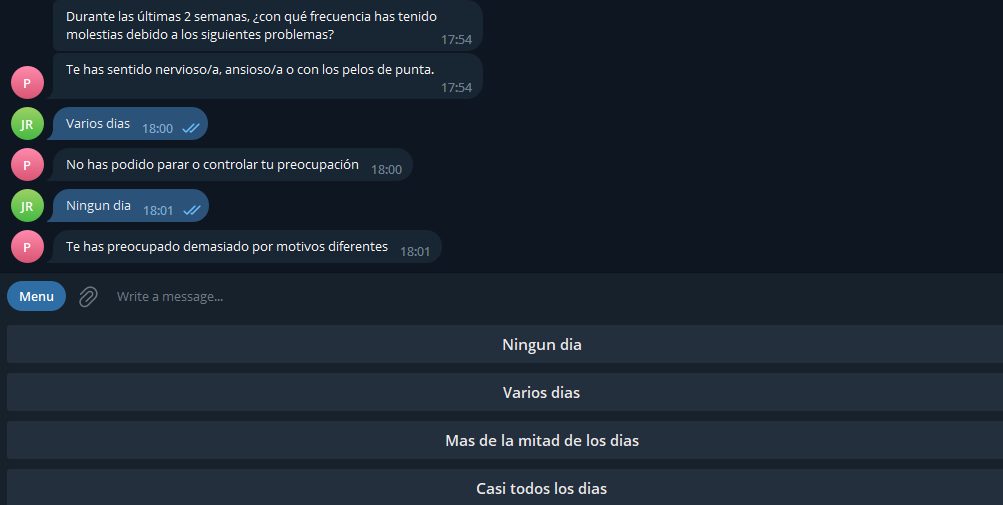
\includegraphics[width=1\textwidth, height=7cm]{imagenes/question.png}
    \caption{ Cuestionario }
    \label{fig:cuestionario}
\end{figure}

Ya sabemos que cada pregunta cuenta con posibles respuestas de forma independiente. El bot cuando hace la pregunta nos actualiza el teclado de Telegram y nos da la opción solo de contestar mediante botones que contienen las respuestas a la pregunta. Esto se hace de la siguente manera:

\begin{lstlisting}[language=Python]
#Function to get a custom keyboard in Telegram
def custom_keyboard(values):
    schema = [[str(value)] for value in values]
    return ReplyKeyboardMarkup(schema, one_time_keyboard=True, resize_keyboard=True)
\end{lstlisting}

El parámetro pasado contiene las respuestas a la pregunta y haciendo uso de la función \textit{ReplyKeyboardMarkup()} proporcionada por la libreria de Telegram creamos un teclado personalizado con los valores que deseemos. Solo podemos responder a la pregunta si el mensaje esta dentro de estas respuestas. Esto se ha hecho para asegurarnos que los datos obtenidos son correctos y reales, ya que si respondemos cualquier cosa que no tuviera nada que ver se guardaría como respuesta a la pregunta. Por lo que en cada iteracción de la función se comprueba si el mensaje proporcionado por el usuario es válido. En caso negativo, como se muestra en la \textit{\hyperref[fig:wrong]{figura 5.6}} el bot no pasaría a la siguiente pregunta y volverá a realizarla de forma indefinida hasta que se responda de forma correcta. \vspace{0.3cm}

\begin{figure}[!ht]
    \centering
    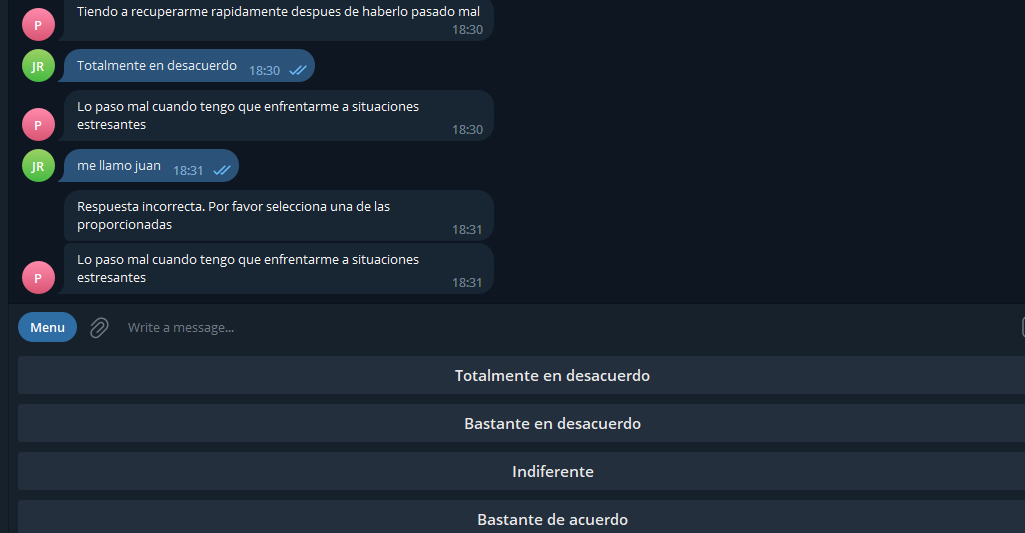
\includegraphics[width=1\textwidth]{imagenes/pregunta_incorrecta.png}
    \caption{ Respuesta incorrecta }
    \label{fig:wrong}
\end{figure}\vspace{0.3cm}

Solo cuando esta sea correcta guardará la respuesta en la base de datos. La función finaliza cuando el usuario haya terminado de responder todas las preguntas y te redirigirá de forma automática al módulo conversacional creando un Job para el usuario que te avisará cuando cuentes de nuevo con preguntas pendientes. \vspace{0.5cm}

\begin{figure}[!ht]
    \centering
    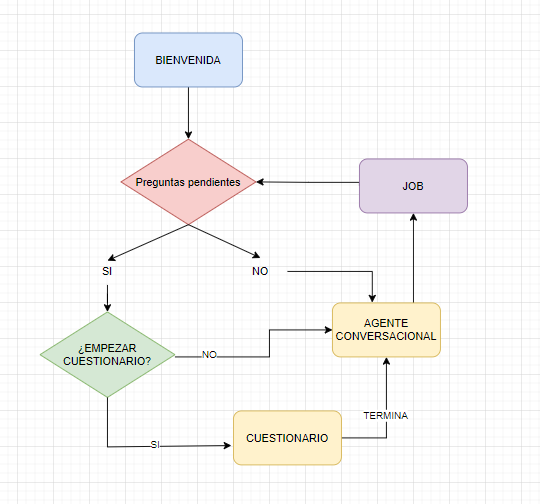
\includegraphics[width=1\textwidth]{imagenes/flujo.png}
    \caption{ Diagrama de flujo del bot}
    \label{fig:flujo}
\end{figure}

En la \textit{\hyperref[fig:flujo]{figura 5.7}} se ve como sería el diagrama de flujo que sigue el bot y la lógica que utiliza. Recapitulando todo el proceso, cuando se inicie una conversación con el bot, este te registrará en la base de datos como un nuevo usuario. Comprobará si se tiene preguntas, en caso afirmativo se empezará realizando el cuestionario que se encuentre activo para tí en ese momento y cuando se termine te llevará al módulo conversacional en el que se puede charlar con el bot. Cuando el sistema identifique que tienes preguntas pendientes te lo hará saber con un mensaje que se manda automáticamente cada 24 horas y que solo termina cuando se vuelvan a responder.
%
%\chapter{Aplicación Web}

La aplicación web se ha creado con el objetivo de proporcionar una interfaz atractiva y manejable usada como panel de administración de forma que podamos interactuar con los cuestionarios, respuestas e información mostrada en el bot. Esta solución garantiza la integridad y el almacenamiento seguro de los datos almacenados en una base de datos centralizada. 

La aplicación web funciona como intermediario entre el usuario y el bot. Esta se encarga de la creación de cuestionarios, del procesamiento y visualización de las repuestas de manera organizada, lo que facilita su posterior análisis. Nace como solución a satisfacer la importancia de la automatización y agilidad en la recopilación de datos, logrando un enfoque integral para la administración y respuestas de usuarios.

El chatbot se ha pensado para ser utilizado por los usuarios. Sin embargo, la aplicación solo podrá ser usada por el administrador o las personas autorizadas para su uso. En este capítulo explicaré los pasos seguidos para su desarrollo.


\section{Arquitectura} 


Django es un framework basado en el modelo  MVC (Model-View-Controller). MVC es un patrón arquitectónico que separa una aplicación en tres componentes lógicos principales: el modelo, la vista y el controlador. Cada uno de estos componentes está diseñado para manejar aspectos de desarrollo específicos de una aplicación. Además, MVC es uno de los marcos de desarrollo web estándar de la industria más utilizados para crear proyectos escalables y extensibles.

Django implementa este patrón MVC de una manera peculiar y con algunas variaciones que ellos llaman MTV, que viene siendo la de Model, Template, View \textit{(\cite{djangomvt})}.

\begin{itemize}

\item M significa "Model" (Modelo), la capa de acceso a la base de datos. Esta capa contiene toda la información sobre los datos: cómo acceder a estos, cómo validarlos, cuál es el comportamiento que tiene, y las relaciones entre los datos.

\item T significa "Template" (Plantilla), la capa de presentación. Esta capa contiene las decisiones relacionadas a la presentación: como algunas cosas son mostradas sobre una página web u otro tipo de documento.

\item V significa "View" (Vista), la capa de la lógica de negocios. Esta capa contiene la lógica que accede al modelo y la delega a la plantilla apropiada: puedes pensar en esto como un puente entre el modelos y las plantillas.

\end{itemize}

Esta es la lógica seguida para el desarrollo. Si nos adentramos en el codigo, vemos que existe una carpeta llamada \textit{'applications'} que contiene varias subcarpetas y en la que cada una es una tabla diferente en la base de datos. Dentro de estas subcarpetas es donde estan creadas las operaciones relacionadas con los modelos y las vistas. En un nivel superior encontramos la carperta \textit{'templates'}, que incluye las plantillas que dan funcionalidad a estas vistas, tambien separadas por modelos. Y por último dentro de la carpeta \textit{'static'} se encuentran los archivos que dan apariencia a estas plantillas.



\section{Login}


\begin{figure}[!ht]
    \centering
    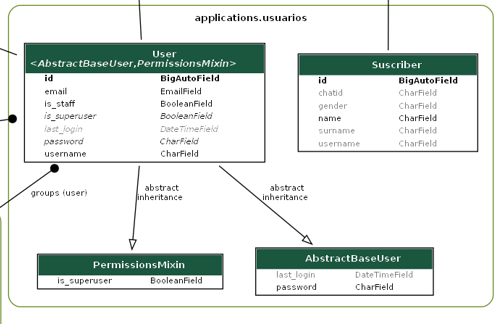
\includegraphics[width=1\textwidth, height=6.5cm]{imagenes/usuarios.png}
    \caption{ Diagrama tabla usuarios }
    \label{fig:usuarios}
\end{figure}

Existen 2 tipos de usuarios en nuestro sistema como vemos en la \textit{\hyperref[fig:usuarios]{figura 6.1}}

El primer usuario, identificado como \textit{User} que actua como administrador, y es el que cuenta con  todos los privilegios para poder acceder y modificar las tablas de la base de datos además de poder acceder al sistema. Y el segundo tipo \textit{Suscriber} que son los usuarios registrados por el bot sin ningún tipo de autoridad. 

En Django, las operaciones asociadas a los usuarios se manejan a través del sistema de autenticación que tiene incorporado. Permite manejar cuentas de usuario, grupos, permisos, inicios y cierres de sesión, reestablecimiento de contraseñas y sesiones de usuario basadas en cookies. Todo esto ya viene implementado por defecto, pero proporciona opciones para reemplazar y así ampliarlo y personalizarlo para satisfacer las necesidades de tu proyecto.

El login, que se ve en la \textit{\hyperref[fig:login]{figura 6.2}}, es la primera página que se muestra cuando intentamos entrar. Solo pueden acceder a la aplicación los usuarios registrados.

\begin{figure}[!ht]
    \centering
    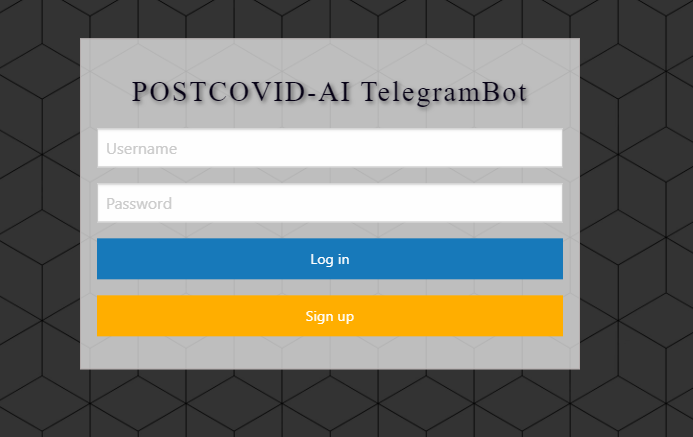
\includegraphics[width=1\textwidth]{imagenes/login.png}
    \caption{ Login usuarios }
    \label{fig:login}
\end{figure}
\vspace{0.8cm}

En caso de no estar registrado se provee de un formulario para ello como se muestra en la \textit{\hyperref[fig:general]{figura 6.3}} . Este rellena los campos de la tabla User que crea un nuevo registro de usuario en el sistema para que pueda autenticarse y acceder a él. Además otorga todos los permisos de administrador para que pueda realizar cualquier tipo de acción. \vspace{0.3cm}


\begin{figure}[!ht]
  \centering
  \begin{subfigure}{0.7\textwidth}
    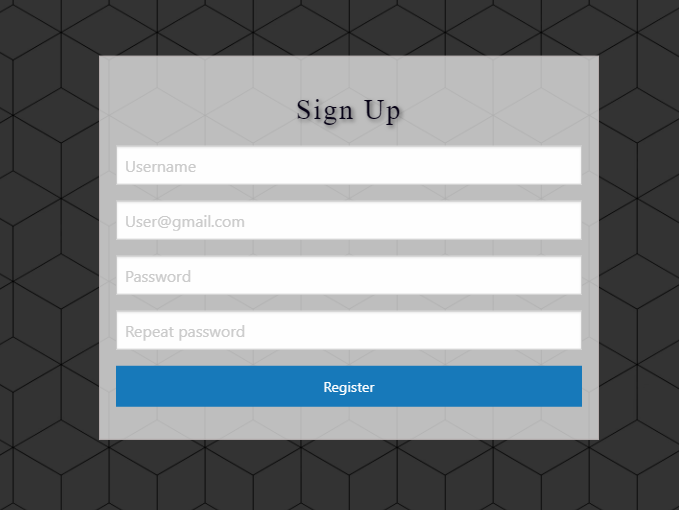
\includegraphics[width=\linewidth]{imagenes/register.png}
    \label{fig:imagen1}
  \end{subfigure}
  \hfill
  \begin{subfigure}{0.7\textwidth}
    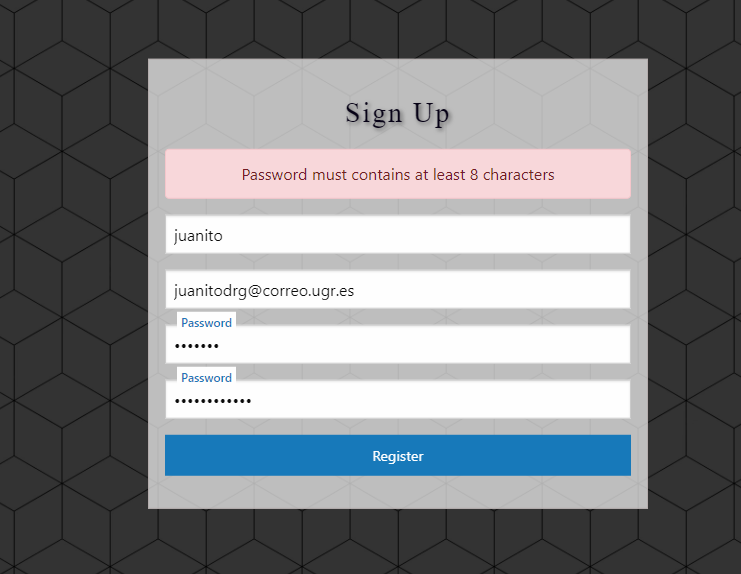
\includegraphics[width=\linewidth]{imagenes/register2.png}
    \label{fig:imagen2}
  \end{subfigure}

  \caption{Formulario de registro}
  \label{fig:general}
\end{figure}\vspace{1cm}

Cada usuario que desee registarse deberá especificar un username, email y la contraseña. El formulario cuenta con validaciones como que el nombre de usuario no se encuentre repetido en el sistema, escribir la contraseña dos veces y que coincidan o que esta tenga más de 8 caracteres. \vspace{1cm}

\section{Home}

Una vez logueados en el sistema, nos redirigirá al home. El home es la vista principal de la aplicación, la primera página que los usuarios ven cuando acceden al sitio web \textit{\hyperref[fig:home]{figura 6.4}}. Proporciona información clave y navegación a otras secciones. Este consta de 4 secciones principales: Preguntas, Bloques, Contextos, Respuestas.\vspace{0.5cm}

\begin{figure}[!ht]
    \centering
    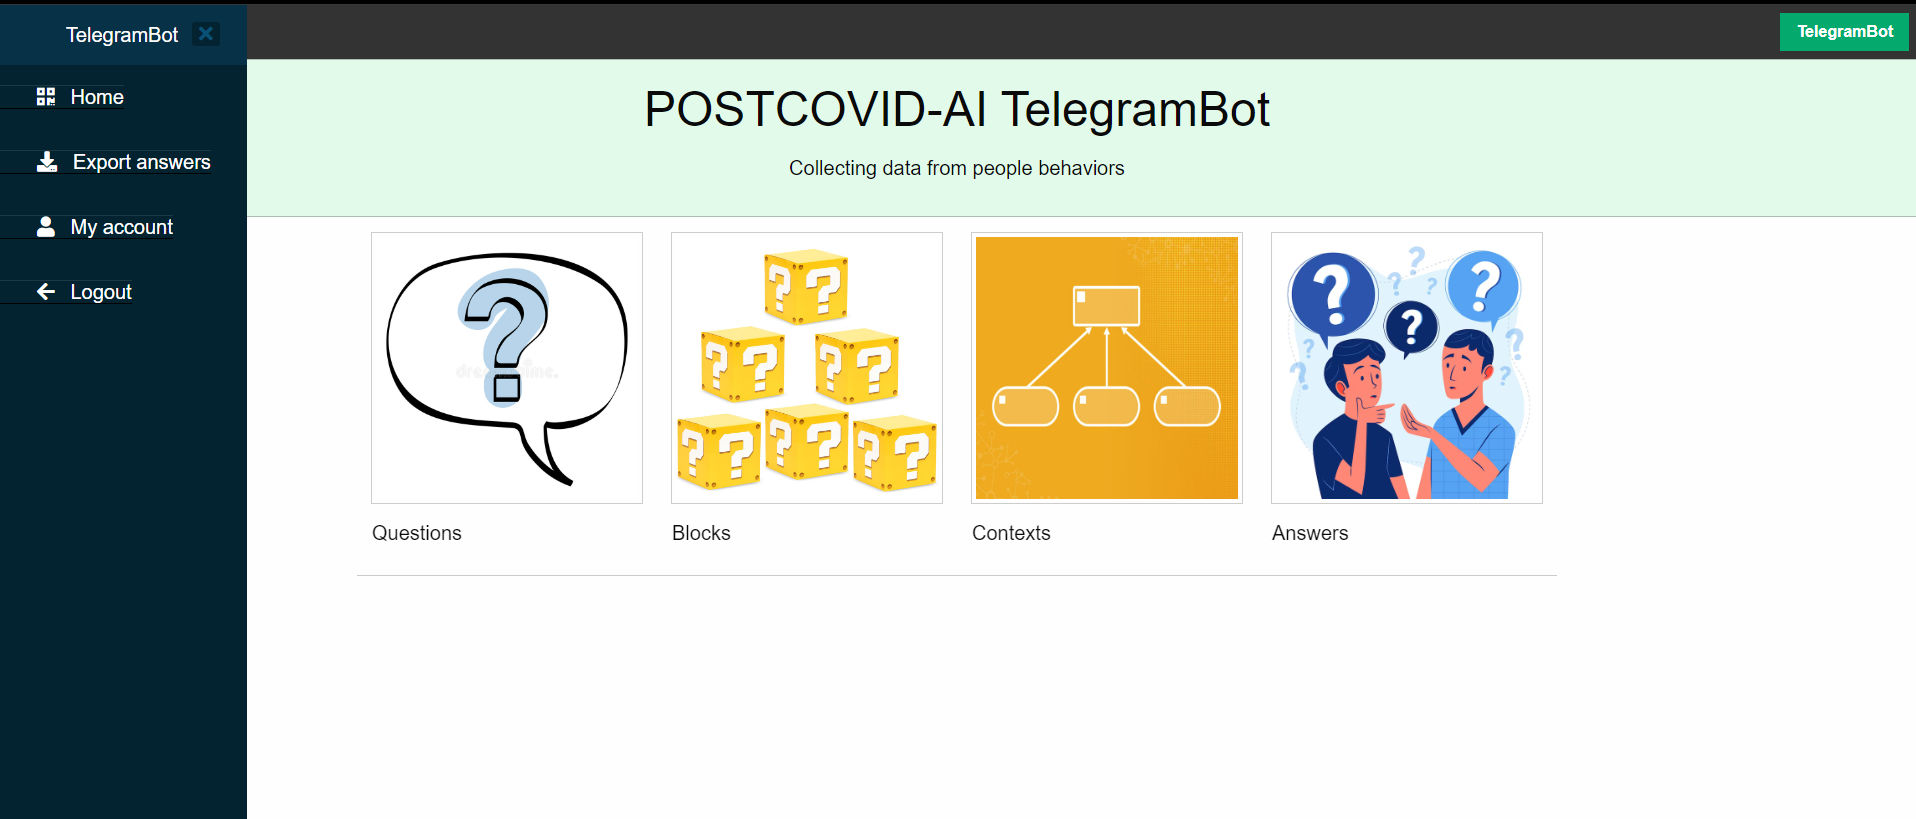
\includegraphics[width=1\textwidth, height=6cm]{imagenes/home.png}
    \caption{ Home }
    \label{fig:home}
\end{figure}
\vspace{0.5cm}

Todas las vistas además cuentan con una barra lateral desplegable para realizar algunas operaciones de manera rápida como exportar respuestas, modificar la información del usuario y hacer logout. 

\begin{figure}[!ht]
    \centering
    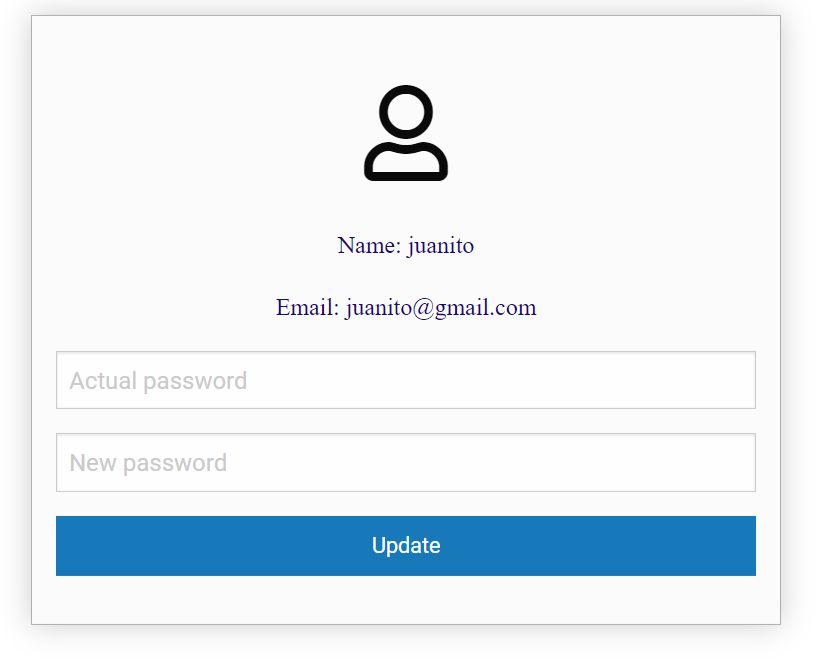
\includegraphics[width=0.5\textwidth, height=5cm]{imagenes/user_update.png}
    \caption{ Actualización usuario }
    \label{fig:modify-user}
\end{figure}

Por ejemplo, en la \textit{\hyperref[fig:modify-user]{figura 6.5}} se muestra la vista de modificar usuario donde nos muestra un formulario con los datos del usuario que se encuentra activo y nos da la posibilidad de cambiar la contraseña, pudiendo proporcionar una nueva.



\section{Gestores}


Todas las secciones que veremos consisten en tablas paginadas que muestran la información guardada de cada registro pertenecientes a cada modelo. Además todas constan de un botón para añadir un nuevo registro, eliminar y otro para modificar. \vspace{0.3cm}

Se ha implementado un buscador en cada una de las vistas de cada sección.

\begin{figure}[!ht]
    \centering
    
\includegraphics[width=0.5\textwidth]{imagenes/search.png}
    \caption{ Buscador }
    \label{fig:enter-label}
\end{figure}

Este buscador mostrará la lista de registros cuyos nombres coincidan con aquello escrito, para facilitar el acceso a la información deseada de manera más eficiente.

\subsection{Preguntas}

\begin{figure}[!ht]
    \centering
    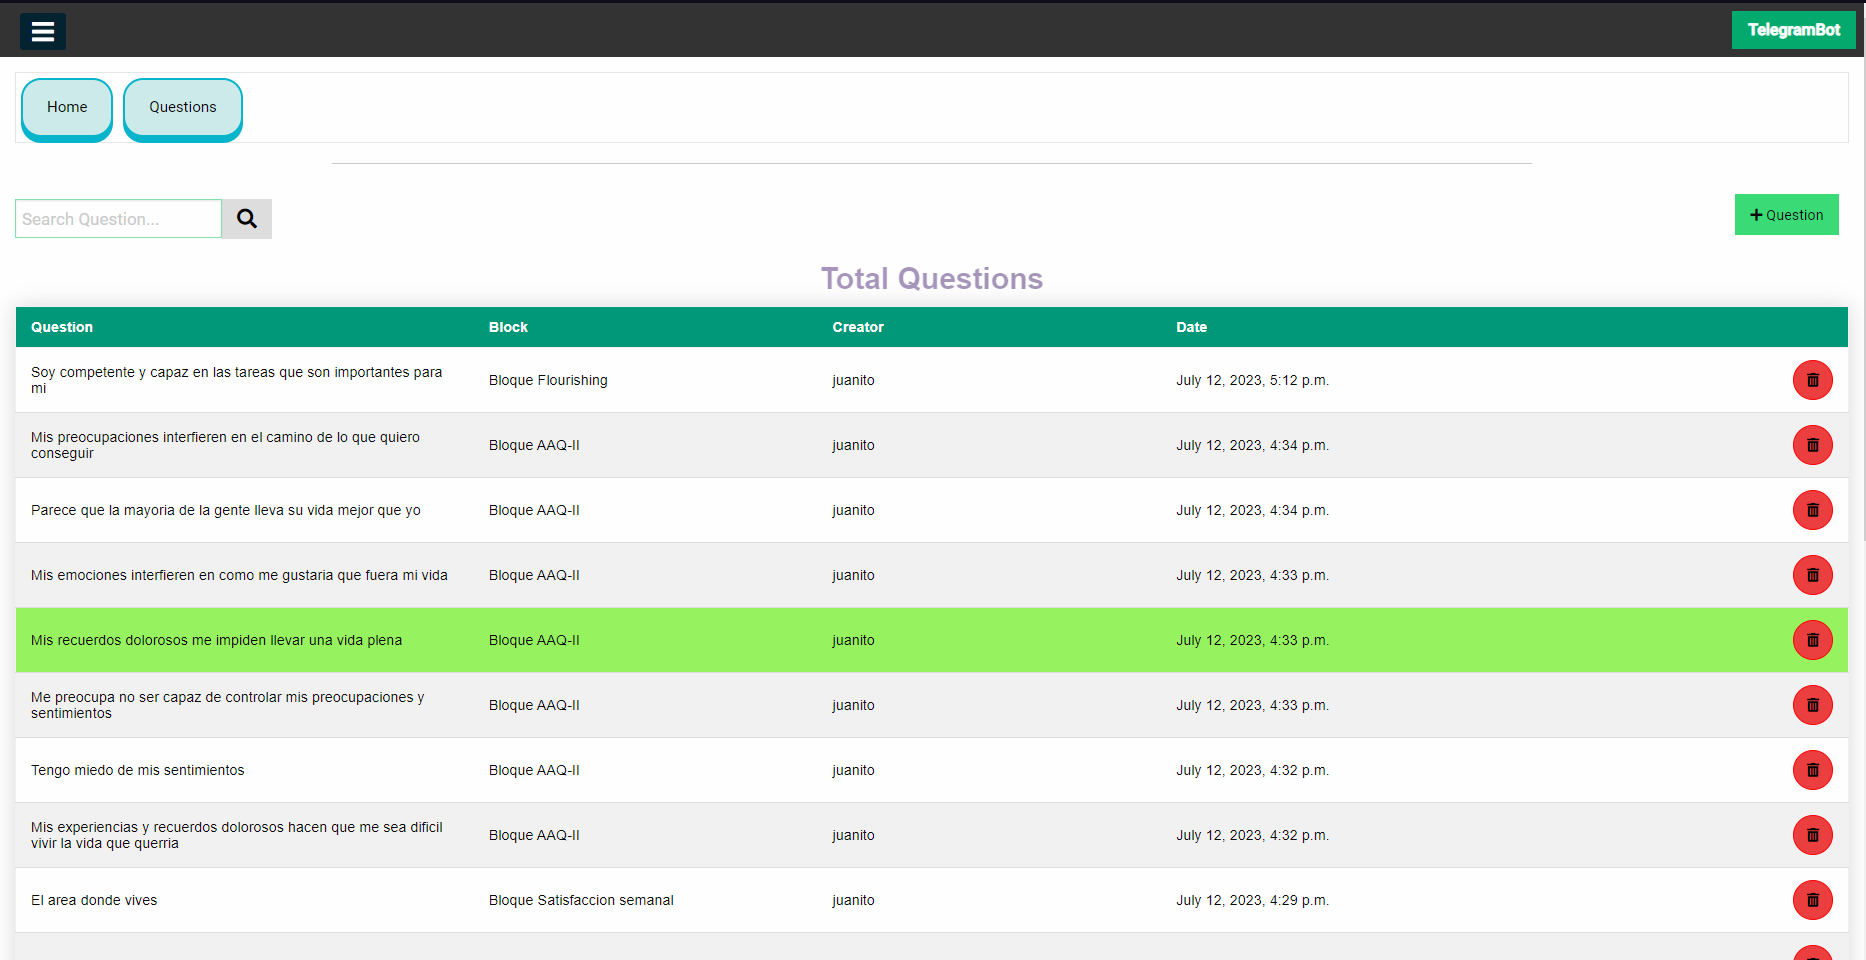
\includegraphics[width=1\textwidth]{imagenes/list_quest.png}
    \caption{ Listado de preguntas }
    \label{fig:vista-preguntas}
\end{figure}\vspace{1cm}

Dentro de la tabla de preguntas se muestra de forma general los campos mas relevantes para distinguirlas, mostrado en la \textit{\hyperref[fig:vista-preguntas]{figura 6.7}}, como el enunciado, el bloque al que pertenecen, la fecha y el usuario que la ha creado. 

Como vemos en la parte superior derecha se encuentra un botón para añadir una pregunta. Si navegamos por las filas de la tabla y clicamos en una se nos abrirá la vista para modificar la pregunta. Además en la parte derecha de cada fila hay un botón para eliminar el registro deseado. 

Si se pulsa en el botón para añadir una pregunta se abrirá una nueva página con un formulario con los datos necesarios para registrarla. 


A nivel de base de datos los campos que requiere cada pregunta son los siguientes:\vspace{0.3cm}

\begin{itemize}
    \item \textit{id}
    \item  \textit{title}: Enunciado de la pregunta.
    \item \textit{creator}: Foreign key a Usuario.
    \item \textit{date}: Fecha en la que se crea la pregunta. 
\end{itemize}\vspace{0.3cm}

El id como en todas las tablas es la clave primaria. A su vez, la pregunta tiene una clave externa a la tabla \textit{Posibles Respuestas}. Por lo que cada pregunta tiene varias posibles respuestas y cada posible respuesta tiene asignada una pregunta. En este caso, como se ve en la \textit{\hyperref[fig:add-question]{figura 6.8}}, para registrar la pregunta solo necesitamos proporcionar el titulo y las posibles respuestas ya que el campo de creador se autorellena con el usuario que la crea y la fecha se pone a la actual.\vspace{1cm}

\begin{figure}[!ht]
    \centering
    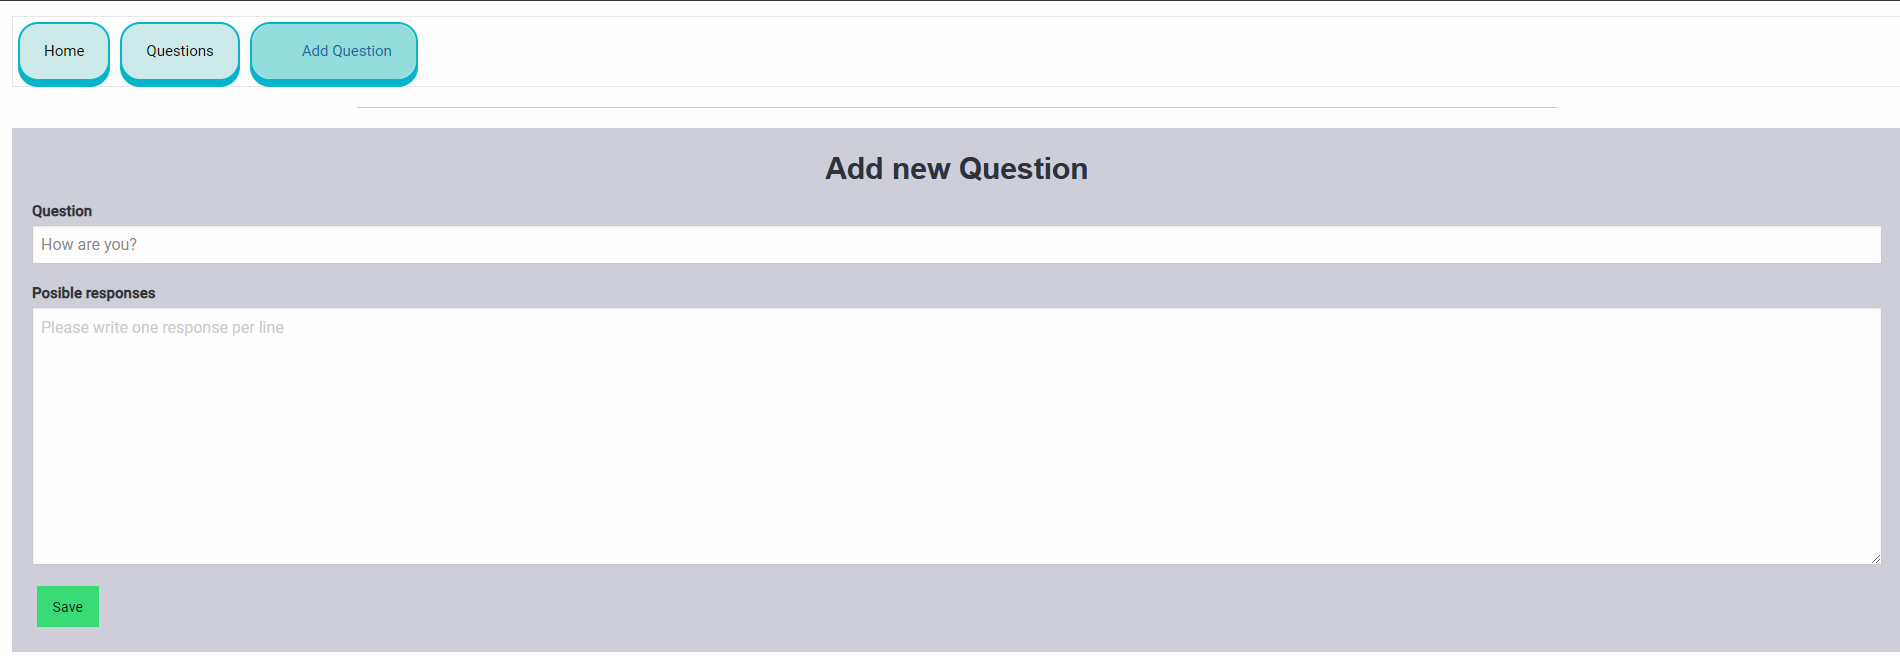
\includegraphics[width=1\textwidth]{imagenes/add_pregunta.png}
    \caption{ Añadir pregunta}
    \label{fig:add-question}
\end{figure}\vspace{1cm}

Dentro del panel de posibles respuestas debemos añadir las respuestas a esa pregunta, cada una separada por línea. A su vez cuando se cree la pregunta también se crearán los registros de las respuestas asociadas a la pregunta. \vspace{1cm}

\begin{figure}[!ht]
    \centering
    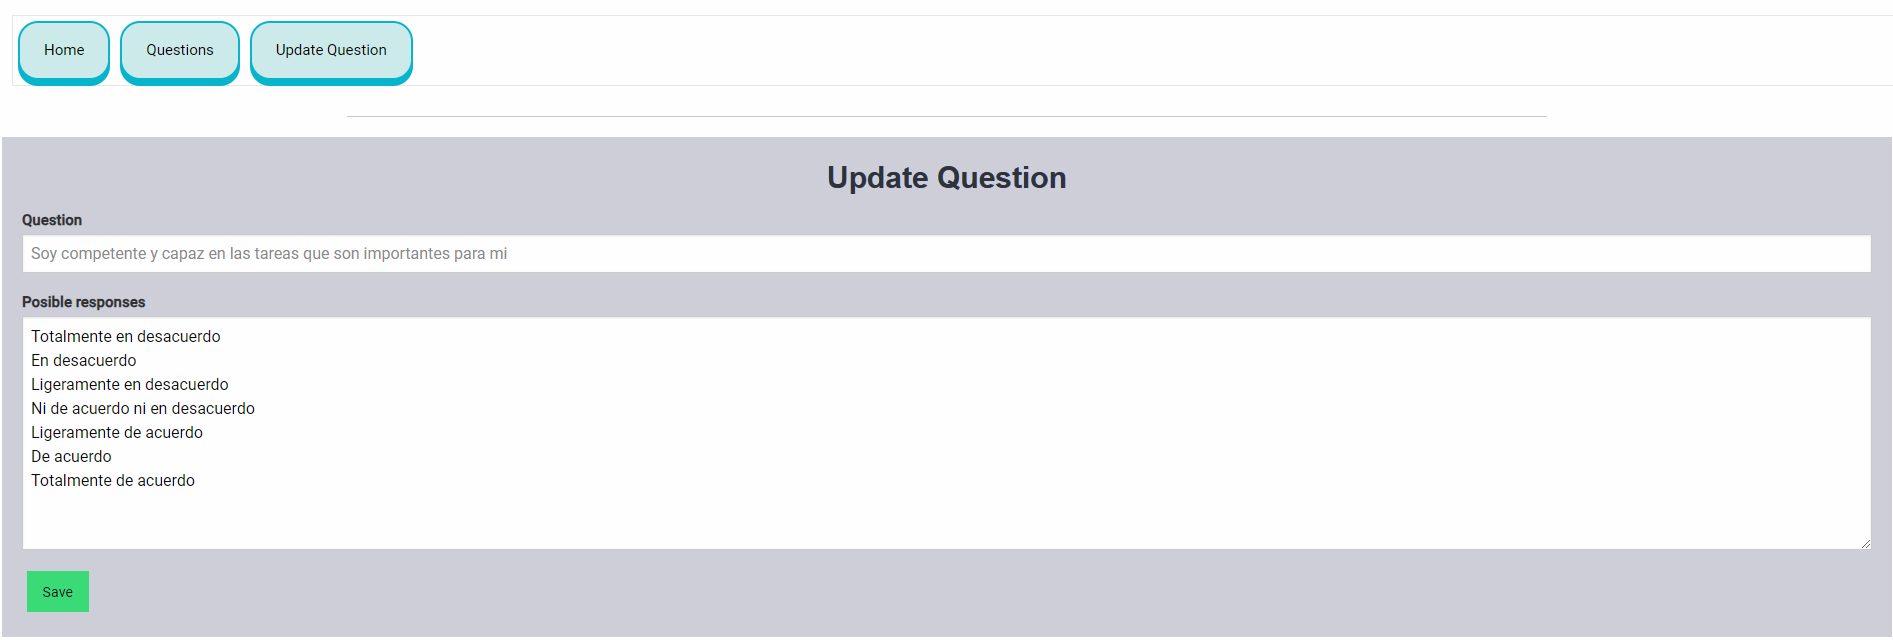
\includegraphics[width=1\textwidth]{imagenes/update_pregunta.png}
    \caption{ Modificar Pregunta}
    \label{fig:modify-question}
\end{figure}\vspace{0.5cm}

En la \textit{\hyperref[fig:modify-question]{figura 6.9}} observamos el formulario de modificación de la pregunta en el que se puede cambiar el titulo y las respuestas. Si otro usuario modifica la pregunta también se actualiza el campo del creador y fecha.

Y por último si se selecciona el botón de eliminar (que se ve como un símbolo de papelera rojo a la derecha de cada fila), aparecerá una alerta para verificar si realmente se desa borrar la pregunta \textit{\hyperref[fig:delete-question]{(figura 6.10)}}.

\begin{figure}[!ht]
    \centering
    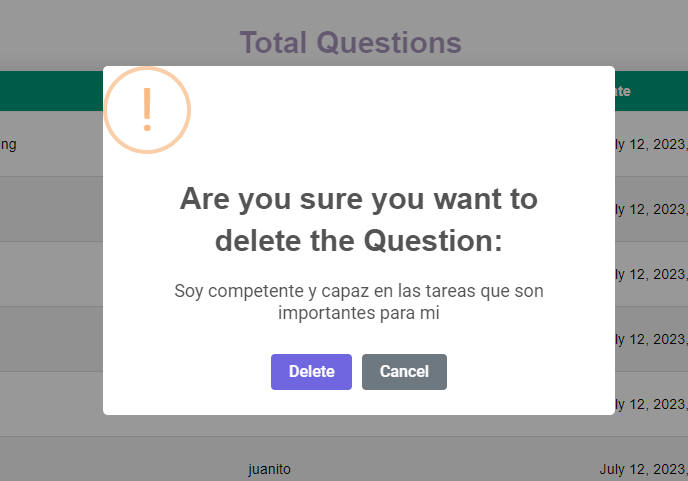
\includegraphics[width=0.7\textwidth, height=7cm]{imagenes/delete_pregunta.png}
    \caption{ Borrar Pregunta}
    \label{fig:delete-question}
\end{figure}\vspace{3cm}



\subsection{Bloques}

\begin{figure}[!ht]
    \centering
    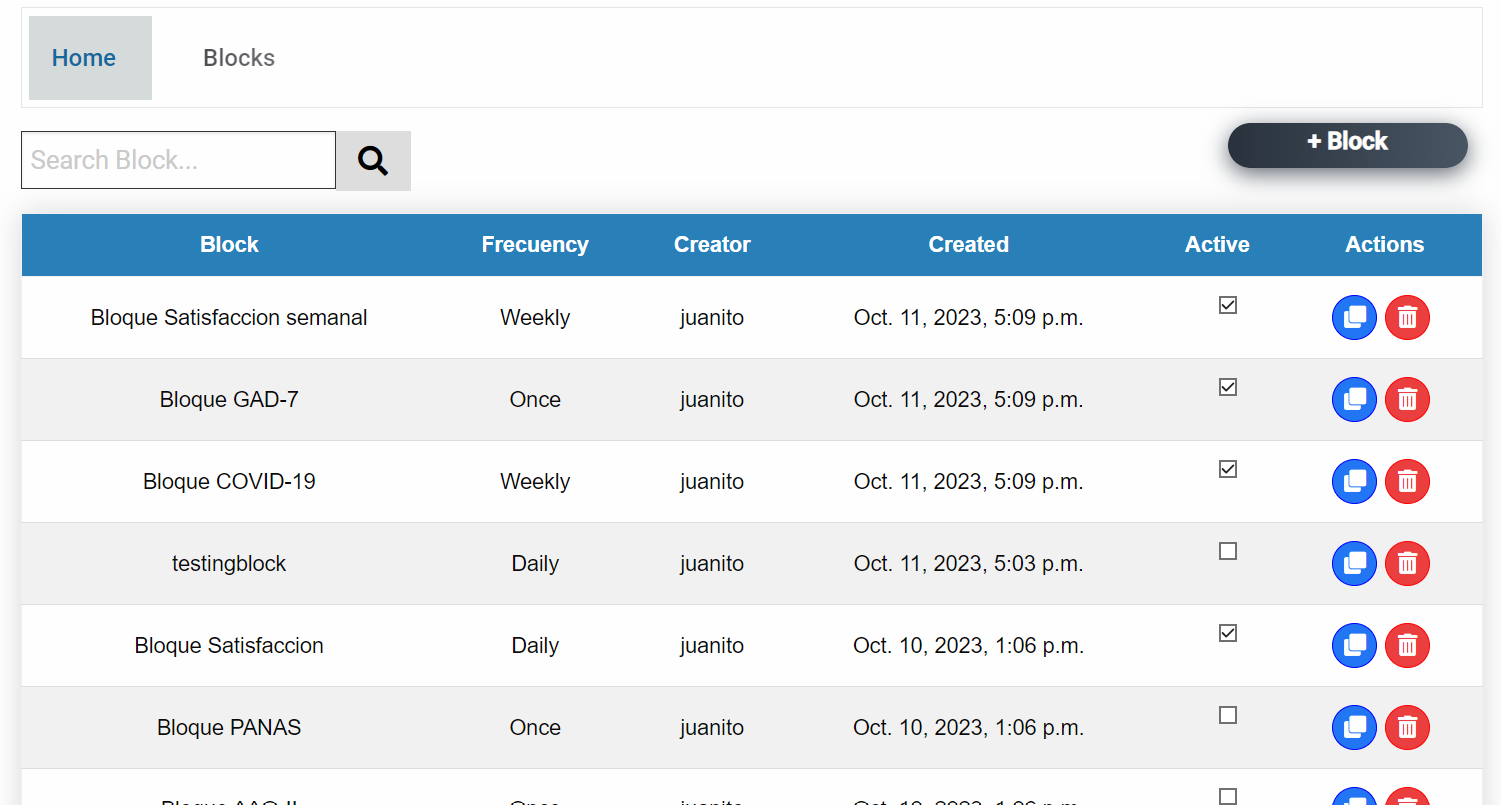
\includegraphics[width=1\textwidth]{imagenes/list_bloques.png}
    \caption{Listado de Bloques}
    \label{fig:lista-bloques}
\end{figure}\vspace{1cm}

La \textit{\hyperref[fig:lista-bloques]{figura 6.11}} muestra la tabla que contiene los registros de los bloques de preguntas en el sistema. Al igual que en la vista anterior cuenta con las operaciones de añadir, modificar y eliminar un bloque. \vspace{0.3cm}

Los campos necesarios para registrar un bloque en la base de datos son los siguientes: \vspace{0.3cm}

\begin{itemize}
    \item \textit{id}
    \item \textit{block}: nombre del bloque.
    \item \textit{active}: atributo booleano que indica si el bloque se encuentra activo.
    \item \textit{questions}: Foreign Key a pregunta.
    \item \textit{context}: Foreign key a contexto.
    \item \textit{frecuency}: Frecuencia del bloque.
    \item \textit{importance}: Importancia del bloque.
\end{itemize}\vspace{0.3cm}

El campo \textit{questions} es una relacion de tipo \textit{ManyToMany} con la tabla de preguntas. Un mismo bloque tendrá la posibilidad de asignar el número de preguntas que desee. Todas esas preguntas a su vez pertenecerán a ese bloque.  

Como vemos en la \textit{\hyperref[fig:add-bloque]{figura 6.12}}, se puede elegir mediante un checkbox las preguntas que se desee añadir y un recuadro en el que  muestra una lista de los contextos creados en el sistema, para elegir uno y asignarlo al bloque. \vspace{0.7cm}


\begin{figure}[!ht]
    \centering
    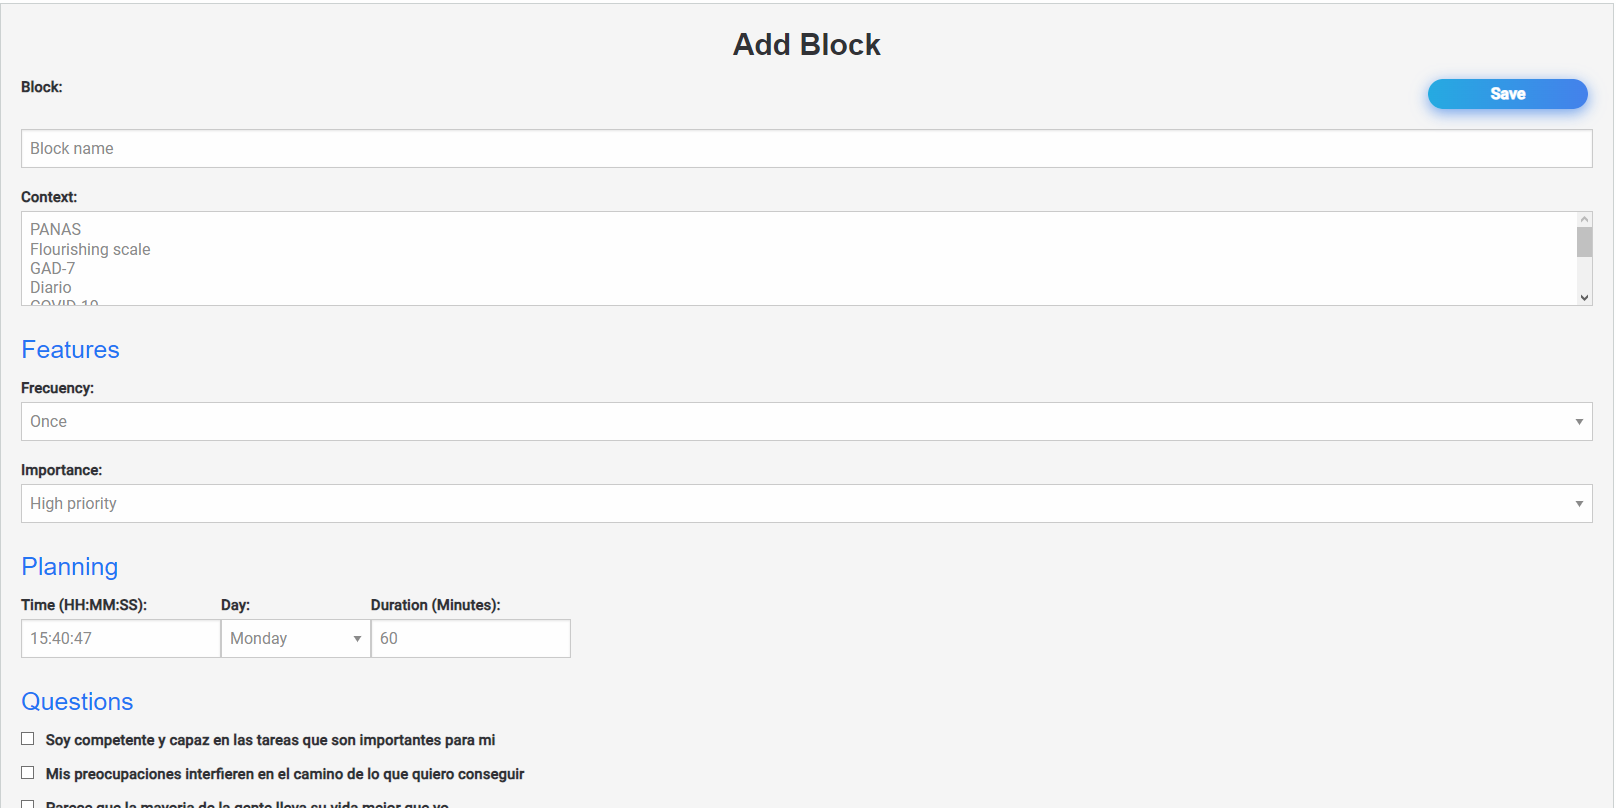
\includegraphics[width=1\textwidth]{imagenes/add_block.png}
    \caption{Añadir bloque}
    \label{fig:add-bloque}
\end{figure}\vspace{0.7cm}

Una vez se han añadido preguntas al bloque y se le ha asignado un contexto, faltaría definir la frecuencia del bloque y su importancia. Estos atributos están más relacionados con el bot. La frecuencia define cada cuanto tiempo se debe realizar el cuestionario asociado al bloque. Normalmente, las preguntas dentro de un mismo bloque tienen un sentido y un propósito común. Por ejemplo, hay preguntas sobre salud, horas de sueño, alimentación que necesitan de realizarse todos los días o una vez por semana. Mientras que hay otras que con solo hacerse una vez ya bastaría. De ahí nace la idea de agrupar las preguntas en bloques. Dentro de la frecuencia puede elegir entre:

\begin{itemize}
    \item Once
    \item Daily
    \item Weekly
    \item Monthly
\end{itemize}

Y como último campo la importancia del bloque (High importance, Normal, Low importance). Este campo  se añadió para que a la hora de que el bot haga el cuestionario de un bloque, priorice los de mayor importancia ante los otros.

\subsection{Contextos}

Los contextos contienen los mensajes a mostrar por parte del bot en el chat del usuario cuando se va a tratar un tema concreto. Cuando se entra en un bloque el bot muestra un mensaje a forma de introducción que nos pone en contexto acerca del tema a tratar en el cuestionario. Esta tabla se crea como idea para que haya variedad a la hora de mostrar estos mensajes introductorios. \vspace{0.7cm}

\begin{figure}[!ht]
    \centering
    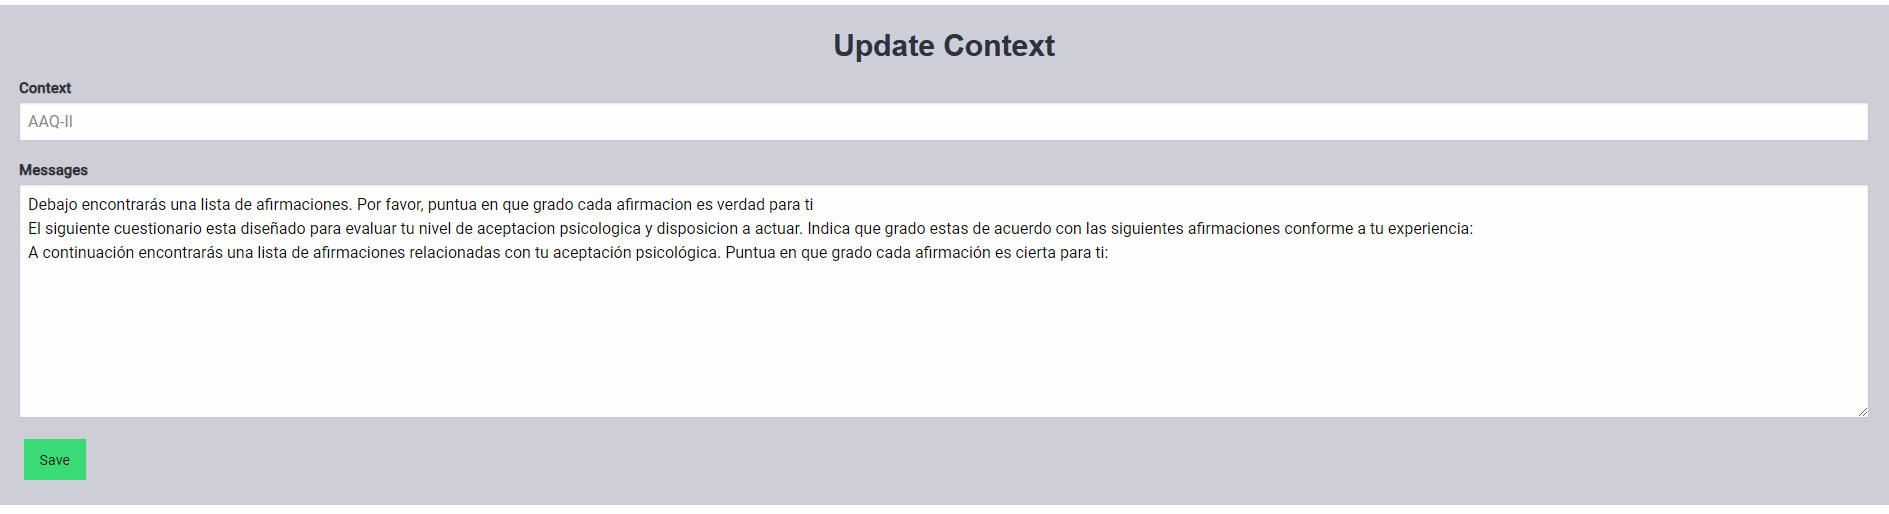
\includegraphics[width=1\textwidth]{imagenes/update_context.png}
    \caption{Editar bloque}
    \label{fig:update-bloque}
\end{figure}\vspace{0.7cm}

En la \textit{\hyperref[fig:update-bloque]{figura 6.13}} se puede ver un ejemplo que nos aclara con mayor detalle la función del contexto. El tema es AAQ-II, estas preguntas sirve para evaluar el nivel de aceptación psicológica y disposición a actuar de una persona. Cuando se realice el cuestionario asociado se mostrará uno de los tres mensajes que dispone. 

La forma de crearlos es parecida a la de las preguntas que se explica previamente. Existen 2 tablas: \textit{Contextos} y \textit{Mensajes}. La clase contexto contiene los nombres, y la de mensajes los enunciados de la información a mostrar, que tienen una clave foránea a contexto. 

\textbf{Clase Contexto:}

\begin{itemize}
    \item \textit{name}: Nombre.
\end{itemize}

\textbf{Clase Mensaje}

\begin{itemize}
    \item \textit{text}: Enunciado del mensaje.
    \item \textit{context}: Foreign key a Contexto.
\end{itemize}


Para crearlo se especifica el nombre y los mensajes, cada uno separado por una línea, que crea todos los registros y los asocia al contexto actual.\vspace{0.5cm}

\subsection{Respuestas}

Por último nos encontramos el apartado de respuestas, mostrado en la \textit{\hyperref[fig:list-answers]{figura 6.14}}. Esta vista es simplemente a modo de visualización ya que el administrador no podrá realizar operaciones con ellas. Estas se crean automáticamente cuando un usuario responde a la pregunta hecha por el bot. \vspace{1cm}

\begin{figure}[!ht]
    \centering
    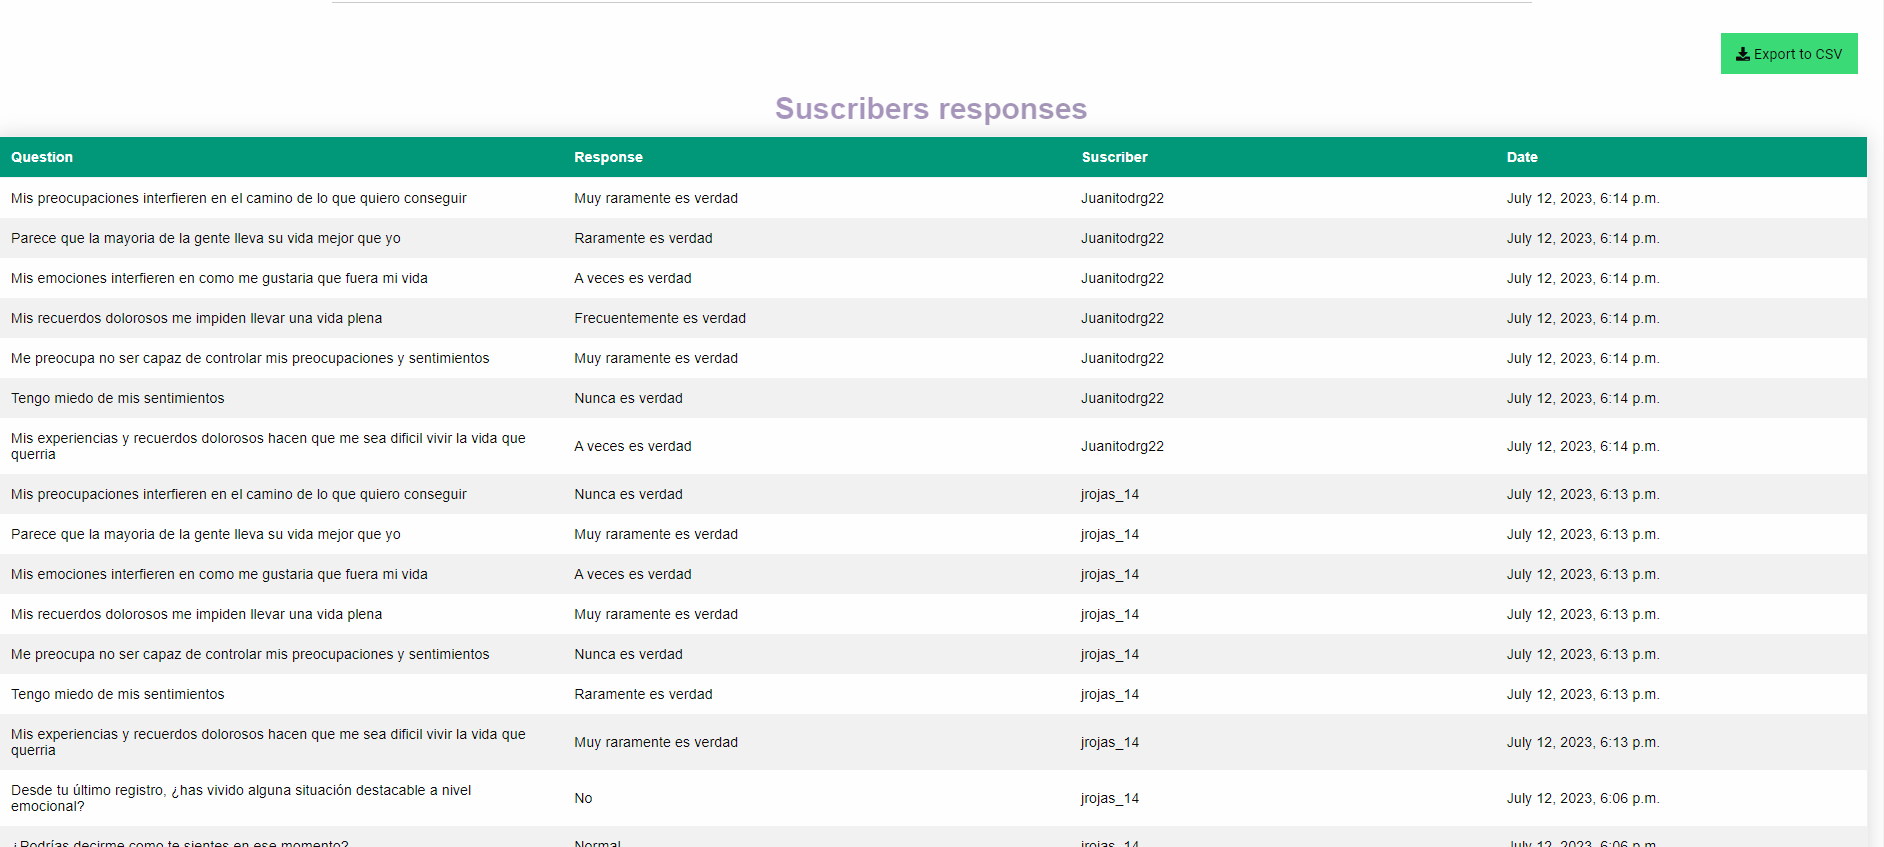
\includegraphics[width=1\textwidth]{imagenes/list_answers.png}
    \caption{Lista respuestas}
    \label{fig:list-answers}
\end{figure}\vspace{0.5cm}



Los campos para registar una respuesta son los siguientes:

\begin{itemize}
    \item \textit{id}
    \item \textit{question}: Foreign key a pregunta.
    \item \textit{response}: Respuesta del usuario.
    \item \textit{suscriber}: Foreign key a usuario.
    \item \textit{date}: Fecha de la respuesta.
\end{itemize}

Esta vista cuenta además con un botón en la parte superior derecha para exportar las respuestas a formato CSV. Los archivos CSV almacenan los datos separados con comas, por lo que cuando se guarda el texto y los números es fácil moverlos de un programa a otro. Al fin y al cabo este es el propósito de nuestro proyecto, recaudar información y entregarla en un formato específico para que el análisis sea sencillo.\vspace{1cm} 

La función que lo realiza es la siguiente:

\begin{lstlisting}[language=Python]
def export_to_csv(request):
    answers = Answer.objects.all()
    response = HttpResponse('text/csv')
    response['Content-Disposition'] = 'attachment; filename=answers_export.csv'
    writer = csv.writer(response)
    writer.writerow(['Question', 'Response', 'Suscriber', 'Date'])
    answer_fields = answers.values_list('question__title', 'response', 'suscriber__username', 'date')
    for answer in answer_fields:
        writer.writerow(answer)
    return response
\end{lstlisting}

Python cuenta con una librería llamada csv. Esta librería implementa clases para leer y escribir datos tabulados en formato CSV.
%
\chapter{Despliegue e instalación}\vspace{1cm}


\section{Despliegue}

El despliegue del proyecto se ha realizado en un repositorio público de mi cuenta de \href{https://github.com/juantiog22}{GitHub}, en el que encontramos todo el código disponible. \vspace{0.3cm}

Para la creación del bot y que se encuentre activo para todo aquel que quiera conversar se ha utilizado la API de Telegram. La aplicación de mensajería pone a disposición de cualquier usuario la creación de bots en su plataforma de manera relativamente sencilla con la ayuda de su robot \textit{BotFather}. Se trata de un bot disponible en cualquier versión de Telegram, escritorio o app móvil, y que se encarga de controlar otros bots. Gracias a la API de que dispone Telegram para bots vamos a poder acceder a una gran cantidad de herramientas que nos ayuda a la hora de desarrrollar la lógica de nuestro bot. Para ello debemos bucar a \textit{@BotFather} en el buscador de Telegram y empezar una conversación con él. Este es el bot oficial que te permitirá crear y administrar tus propios bots. 

Como observamos en la \textit{\hyperref[fig:creacion-bot]{Figura 6.1}}, escribiendo el comando /newbot iniciamos el proceso de creación. Nos solicitará que elijamos un nombre, que será el mostrado en las conversaciones, y un username que deberá de terminar en \_bot o Bot. Una vez creado, nos proporcionará un token de acceso único para nuestro bot. Este es el token con el que vamos a interactuar con la API de Telegram. \vspace{2cm}

\begin{figure}[!ht]
    \centering
    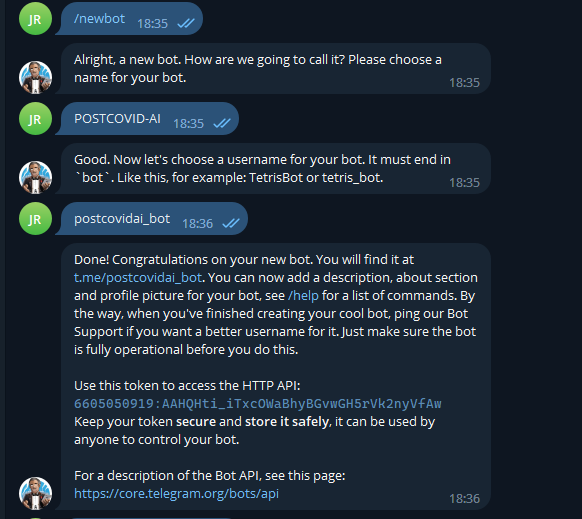
\includegraphics[width=0.7\textwidth, height=7.5cm]{imagenes/bot_creation.png}
    \caption{ Creación del bot en Telegram }
    \label{fig:creacion-bot}
\end{figure}


Hecho esto, tal como se muestra en la \textit{\hyperref[fig:customize-bot]{Figura 6.2}}, podemos personalizar nuestro bot como deseemos, cambiando la descripción, el estado, la foto de perfil, comandos personalizados...

\begin{figure}[!ht]
    \centering
    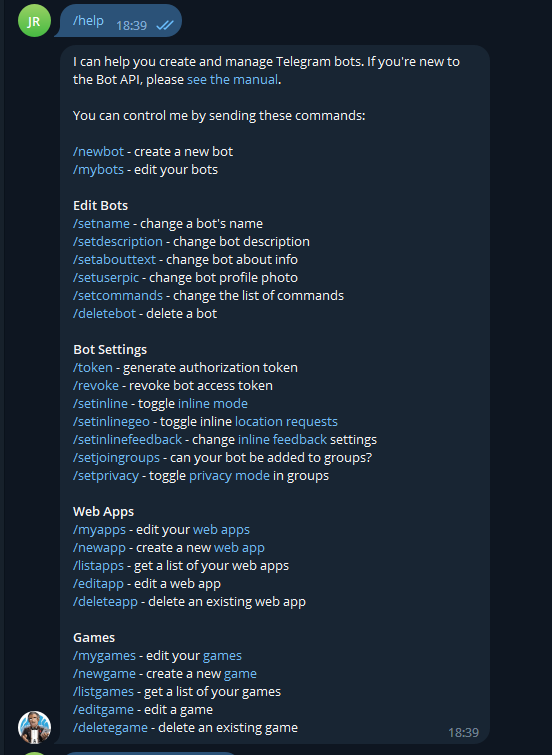
\includegraphics[width=0.8\textwidth, height=8.5cm]{imagenes/bot_custom.png}
    \caption{ Customización del bot }
    \label{fig:customize-bot}
\end{figure}



\section{Instalación}

\subsection{Configuración del entorno}

Antes de explicar como montar el proyecto, son necesarias tener instaladas previamente algunas tecnologías.
La primera de ella es Docker. Dependiendo del sistema operativo que estemos utilizando, debemos descargarlo de una forma u otra. En el caso de Windows, desde la documentación oficial  \textit({\cite{docker})}, nos permite descargar un archivo ejecutable que nos hará la instalación de manera automática. En caso de usar Linux, podemos descargarlo usando los siguientes comandos:

\begin{minted}{bash}
    $ sudo apt-get update
    $ sudo apt-get install ca-certificates curl 
    $ sudo install -m 0755 -d /etc/apt/keyrings
    $ curl -fsSL https://download.docker.com/linux/ubuntu/gpg | sudo gpg 
    --dearmor -o /etc/apt/keyrings/docker.gpg
    $ sudo chmod a+r /etc/apt/keyrings/docker.gpg
    $ echo \
      "deb [arch="$(dpkg --print-architecture)" signed-by=/etc/apt/keyrings/
      docker.gpg] https://download.docker.com/linux/ubuntu \
      "$(. /etc/os-release && echo "$VERSION_CODENAME")" stable" | \
      sudo tee /etc/apt/sources.list.d/docker.list > /dev/null$
    $ sudo apt-get update
    $ sudo apt-get install docker-ce docker-ce-cli containerd.io 
    docker-buildx-plugin docker-compose-plugin
\end{minted}

El lenguaje de programación utilizado es python, por lo que debemos de tenerlo descargado y declarado como variable de entorno en nuestro sistema. En su página oficial, explica como hacerlo \textit({\cite{python})}

El gestor de base de datos utilizado es PostgreSQL. También es posible descargarlo en Windows utilizando el instalador que proveen \textit({\cite{postgres})} o en el caso de Linux ejecutando los siguientes comandos:

\begin{minted}{bash}
    $ sudo sh -c 'echo "deb http://apt.postgresql.org/pub/repos/apt
    $(lsb_release -cs)-pgdg main" > /etc/apt/sources.list.d/pgdg.list'
    $ wget --quiet -O - https://www.postgresql.org/media/keys/ACCC4CF8.asc 
    | sudo apt-key add -
    $ sudo apt-get update
    $ sudo apt-get -y install postgresql
\end{minted}


\subsection{Montaje de desarrollo}

Una vez tengamos todo lo necesario, ya podemos pasar al montaje del proyecto. Para ello, descargamos el código del repositorio público de github que contiene el proyecto. Podemos hacerlo a mano o mediante comando.

\begin{minted}{bash}
    $ git clone https://github.com/juantiog22/Thesis.git
\end{minted}

Se ha usado Docker ya que permite entregar código con mayor rapidez, estandarizar las operaciones de las aplicaciones, transferir el código con facilidad y ahorrar dinero al mejorar el uso de recursos. Con Docker, obtiene un solo objeto que se puede ejecutar de manera fiable en cualquier lugar. La sintaxis sencilla y simple de Docker le aporta un control absoluto, por lo que todo lo necesario a la implantación del proyecto ya se encuentra proporcionado. Dentro de la carpeta de \textit{/Thesis} ejecutamos este comando:

\begin{minted}{bash}
    $ docker-compose up -d --build  
\end{minted}

Esto creará las imágenes de docker correspondientes a la interfaz web, el bot y la base de datos. Además instalará todos los paquetes necesarios situado dentro del archivo \textit{'requirements.txt'}. 
Para la creación de la base de datos, se ha exportado una por defecto que se encuentra dentro del archivo \textit{'dumpfile.sql'}. Esta base de datos cuenta con preguntas, bloques y preámbulos previamente creados con ejemplos reales de como serían algunos cuestionarios guiándome según las reglas e información relevante que me proveen desde \textit({\cite{postcovid})}. En el caso de querer establecer esta base de datos tras haber hecho el paso anterior debemos restaurar la nuestra con la información que contiene este archivo. Para ello:

\begin{minted}{bash}
    $ docker-compose exec db bash
    $ pg_restore -U postgres -d postgres /var/lib/postgres/data
    /dumpfile.sql
\end{minted}

Esto vuelca toda la información en nuestra base de datos y migrará todos los datos de forma automática en la base de datos que provee PostgreSQL por defecto. En el caso de no querer usar esa base de datos y querer crear otra nueva pero con todos los cambios debemos de crearla previamente. Desde la terminal de psql podemos hacerlo con el siguiente comando:

\begin{minted}{bash}
    $ createdb -U "nombre_propietario" "nombre_base_datos"
\end{minted}

Si hacemos esto, debemos hacer un par de cambios antes de la instalación. En el archivo \textit{'docker-compose.yml'}, podemos cambiar las variables relacionadas con el entorno de la base de datos antes de construir la imagen.

\begin{minted}{bash}
    - POSTGRES_USER=postgres
    - POSTGRES_DB=postgres
    - POSTGRES_PASSWORD=postgres
\end{minted}

También dentro de la ruta \textit{'/telegrambot/telegrambot/settings/local.py'} es donde se define la base de datos con la que vamos a trabajar, podemos cambiarlo modificando los parámetros como deseemos. 


\begin{minted}{Python}
DATABASES = {
    'default': {
        'ENGINE': 'django.db.backends.postgresql',
        'NAME': 'postgres',
        'USER': 'postgres',
        'PASSWORD': 'postgres',
        'HOST': 'db',
        'PORT': 5432,
    }
}
\end{minted}

Tendríamos que cambiar los datos relacionados al usuario, contraseña y nombre. Si queremos crear una base de datos desde cero y completamente nueva, simplemente tras construir la imágenes de docker ejecutamos lo siguiente:

\begin{minted}{bash}
    $ docker-compose run web python manage.py makemigrations
    $ docker-compose run web python manage.py migrate
\end{minted}

Esto generará una base de datos completamente nueva con todas las tablas necesarias, lista para funcionar, aunque estará vacía de registros. Una vez que se haya completado esta fase, ejecutamos el siguiente comando, y nuestro proyecto estará en funcionamiento y preparado para su uso.

\begin{minted}{bash}
    $ docker-compose up
\end{minted}

Es importante asegurarse de que no haya otro proceso corriendo en el mismo puerto a la hora de instalarlo para que no nos encontremos con ningún error. Si desde el navegador accedemos a la url: \textit{http://localhost:8000/} podemos acceder a la aplicación web y además el bot se econtrará escuchando y esperando actualizaciones desde la aplicación de Telegram.
%
\chapter{Conclusiones}

Para concluir nuestro proyecto, vamos a analizar si los requisitos propuestos han sido llevados a cabo. Finalmente expondremos algunos aspectos a mejorar como trabajo futuro y una opinión personal evaluando mi experiencia tras el desarrollo del proyecto. 

\begin{itemize}
    \item Se ha conseguido implementar un chatbot que recoja datos relacionados con el bienestar de las personas.
    \item Se ha conseguido diseñar una arquitectura y una base de datos que cumple con lo que necesitábamos. Tanto la interfaz web, como la base de datos y el bot en telegram se encuentran mutuamente conectados. La base de datos contiene la información  de usuarios, preguntas, bloques, mensajes, respuestas y todo almacenado de forma clara. 
    \item La interfaz web responde adecuadamente a lo que estábamos buscando. Una aplicación sencilla e intuitiva para poder interactuar con el bot y las respuestas recogidas.
    \item El bot es capaz de tener una conversación con el usuario de forma escueta para satisfacer la interacción. Además de realizar el cuestionario cuando sea oportuno.
    \item El almacenamiento de las respuestas en la base de datos se realiza de forma automática y correcta, con la funcionalidad añadida de poder exportarlas.
\end{itemize}

El desarrollo del proyecto se ha alargado algo más de lo planteado, debido a ciertos cambios en el diseño que conforme se ha ido implementado han ido surgiendo, también sumado al desconocimiento de algunas tecnologías usadas. Pero tras tener todo esto en cuenta, el resultado ha sido satisfactorio ya que todo los requisitos planteados han sido cubiertos. 



 \section{Aspectos a mejorar}

La funcionalidad de nuestro proyecto puede ser mejorada de diversas formas. En el caso del bot sobre todo, se puede mejorar el tema de la interacción con el usuario usando sistemas de procesamiento de lenguajes más avanzados. También se podría exportar a otras plataformas y que pueda llegar a más personas. En el caso de la aplicación web un punto potencial de mejora sería la creación de una API que nos permita la interacción con la base de datos de una forma más eficiente. Además de algunos buscadores y filtros por parámetros dentro de las vistas de tablas. 


 \section{Valoración personal}

 Este trabajo ha sido mi mayor reto afrontado en el transcurso de mi etapa como estudiante en la Universidad de Granada al comprometerme para su desarrollo en un entorno de trabajo real. Además sumado a lenguajes, técnicas y áreas donde no tenía especial conocimiento, pero el interés por mi parte a todo tipo de competencia han marcado una etapa de aprendizaje de forma individual bastante enriquecedora. En esta línea, he intentado utilizar siempre cosas útiles y empleadas por programadores y empresas en la actualidad, por lo que todo lo adquirido me ayudará en el desarrollo de futuros proyectos y trayectoria profesional.

 Tras haber realizado este proyecto me he dado cuenta de cómo las tecnologías pueden enriquecer y facilitar nuestras vidas cotidianas. Observamos que la tecnología en sí misma no es un fin, sino un medio para lograr el florecimiento humano. A medida que nos adentramos cada vez más en un mundo más tecnológico, es fundamental reconocer que estas herramientas son manifestaciones de la capacidad humana para imaginar, crear y transformar su realidad. 

\begin{quote}
    \textit{"La tecnología no es nada. Lo importante es que tengas fe en la gente, que sean básicamente buenas e inteligentes, y si les das herramientas, harán cosas maravillosas con ellas."} \\ 
    -- Steve Jobs.
\end{quote}

%
\appendix 

\chapter{Guía de Uso}

En este apéndice, aprenderemos a usar de forma general el proyecto, explicando paso a paso cada funcionalidad, poniendo a prueba algunos casos de uso y examinando la función de cada parte implicada.

\section{Ingreso}

Tras haber explicado todo el proceso de instalación y tecnologías necesarias para montar el proyecto, vamos a explicar como acceder a él. 

Si hemos seguido los pasos previos mostrados en el apartado de instalación, el proyecto ya debería de estar montado, las imágenes en docker ya construidas y la base de datos ya creada y migrada. Para ejecutarlo simplemente desde la carpeta inicial del proyecto abrimos una terminal y escribimos el siguiente comando:

\begin{minted}{bash} 
    $ docker-compose up
\end{minted}

Este comando inicializa los contenedores de docker y ejecuta el proyecto en el entorno local de nuestro ordenador. Para acceder a la aplicación web, debemos de usar un navegador como puede ser Google Chrome y escribimos en el buscador esta dirección : http://localhost:8000/ que abrirá el proyecto en una ventana de nuestro navegador.

Una vez estemos dentro nos aparecerá la vista de inicio de sesión. Como no tenemos usuarios creados, vamos al apartado de registro y creamos un nuevo superusuario con los campos requeridos \textit{\hyperref[fig:vista-registro]{(figura A.1)}} que constará con los permisos para realizar cambios y administrar los datos. \vspace{1cm}

\begin{figure}[!ht]
    \centering
    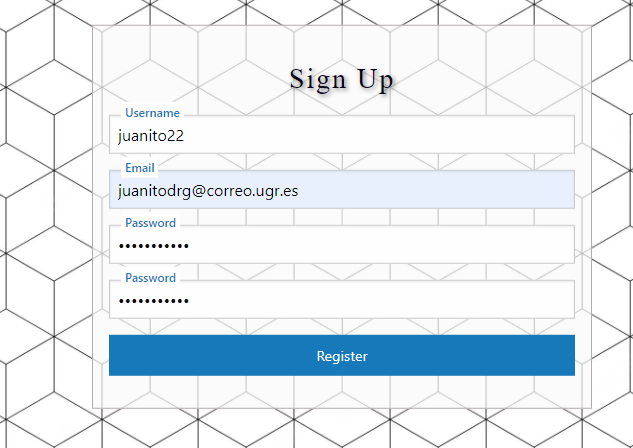
\includegraphics[width=1\textwidth]{imagenes/registro_a.png}
    \caption{ Vista de registro }
    \label{fig:vista-registro}
\end{figure}\vspace{0.5cm}

Una vez registrados, ya podemos hacer login y acceder al panel de administración.\vspace{0.5cm}

\section{Gestión}\vspace{0.5cm}

\subsection{Administración de preguntas}\vspace{0.5cm}

Lo primero de todo es definir las preguntas que queremos que el bot realice a los usuarios. Para ello dentro del apartado de preguntas, en la esquina superior derecha se encuentra la funcionalidad de añadir pregunta. Clicamos y nos abrirá la vista para añadirla. Son necesarios los campos del enunciado y posibles respuestas a la pregunta. 

En la \textit{\hyperref[fig:creacion_pregunta]{figura A.2}} se ve un ejemplo de una pregunta de prueba que he creado. Como vemos le he asignado cuatro posibles respuestas. Se ha añadido también dos preguntas más, cada una con sus respuestas específicas para que luego podamos identificarlas.
\vspace{0.5cm}

\begin{figure}[!ht]
    \centering
    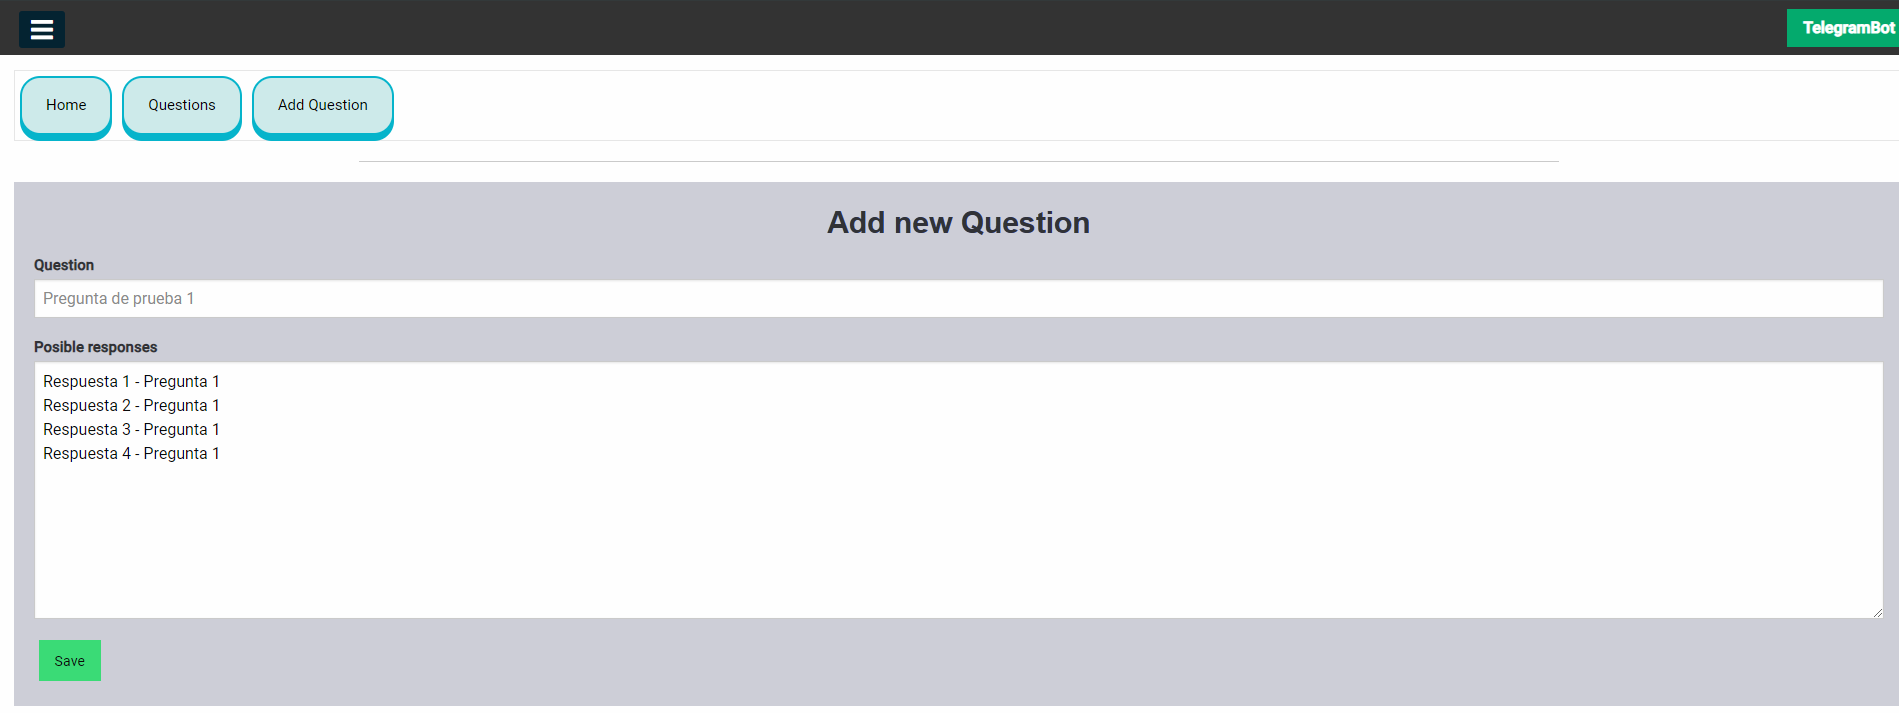
\includegraphics[width=1\textwidth]{imagenes/aniadir_pregunta_a.png}
    \caption{ Vista de creación de pregunta }
    \label{fig:creacion_pregunta}
\end{figure}
 

En la \textit{\hyperref[fig:listado-preg]{figura A.3}} vemos las tres preguntas que acabo de crear con algunos datos relevantes para diferenciarlas. Vemos además que el campo del bloque está vacío, debido a que todavía no tienen ninguno asignado. Si desde aquí clicamos en la fila de la pregunta se nos abrirá una vista para modificar la pregunta o si le damos al icono de la papelera, nos aparecerá un modal para eliminarla.\vspace{0.5cm}

\begin{figure}[!ht]
    \centering
    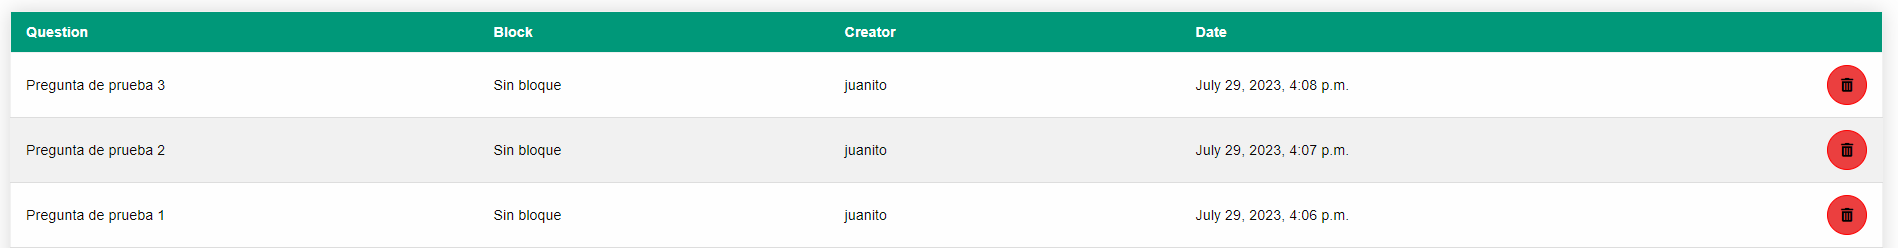
\includegraphics[width=1\textwidth]{imagenes/list_pregunta_a.png}
    \caption{ Vista de listado de preguntas }
    \label{fig:listado-preg}
\end{figure}\vspace{1cm}

\subsection{Administración de Contextos}

Aquí se definirán los contextos, es decir, los mensajes que mostrará el bot cuando haga el cuestionario asociado a un bloque. Para añadirlo, desde la página principal nos dirigimos al apartado de contextos que nos abrirá la vista de los contextos registrados y al igual que antes creamos uno. 

Se crea de igual forma que la pregunta como se ve en la \textit{\hyperref[fig:creacion-contexto]{figura A.4}}, con la diferencia que el primer campo es el nombre del contexto y el segundo los mensajes asociados a él. Cada mensaje deberá ocupar una línea diferente en el formulario. \vspace{2cm}

\begin{figure}[!ht]
    \centering
    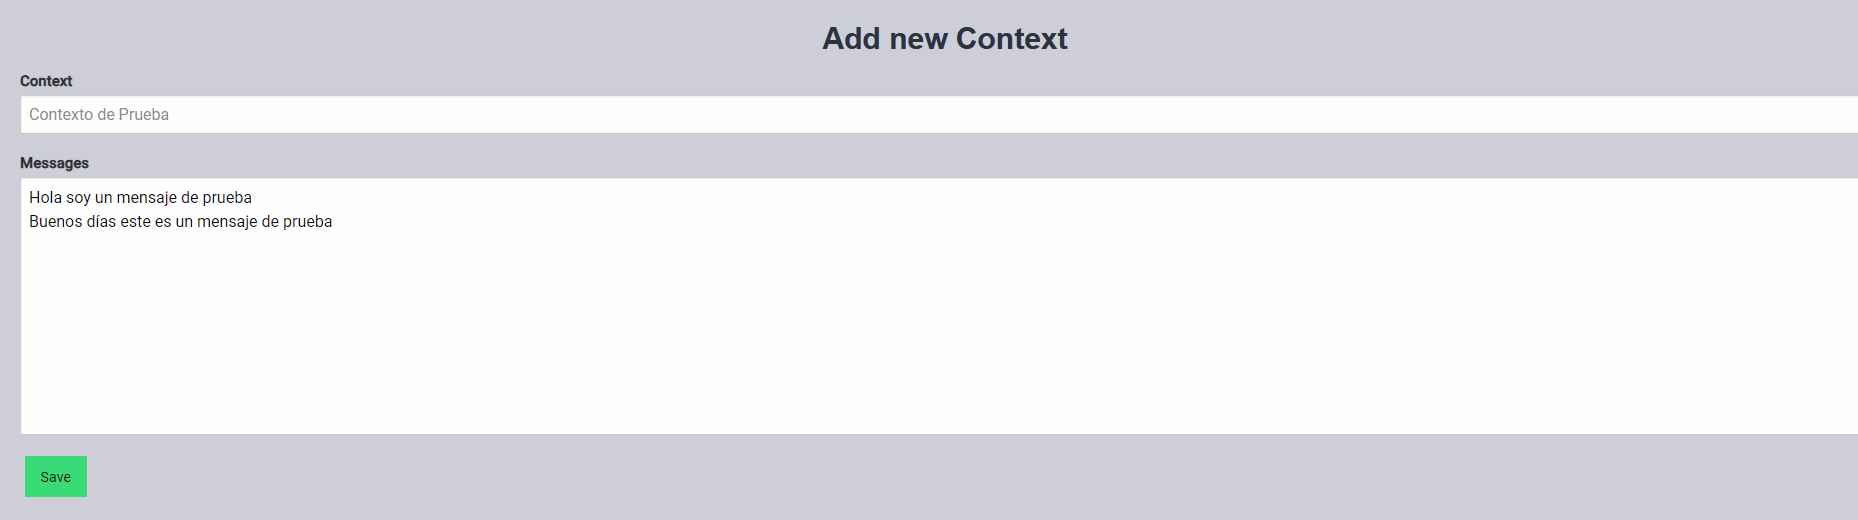
\includegraphics[width=1\textwidth]{imagenes/add_context_a.png}
    \caption{ Vista creación de contexto }
    \label{fig:creacion-contexto}
\end{figure}

\subsection{Administración de Bloques}

Pasamos a la creación de bloques. Al igual que en los ejemplos anteriores en el apartado de bloques, podemos añadir nuevos. Elegimos el nombre, las preguntas que queramos que contenga, el contexto, seleccionamos que este activo y elegimos la frecuencia \textit{\hyperref[fig:creacion-bloques]{figura A.5}}. 

\begin{figure}[!ht]
    \centering
    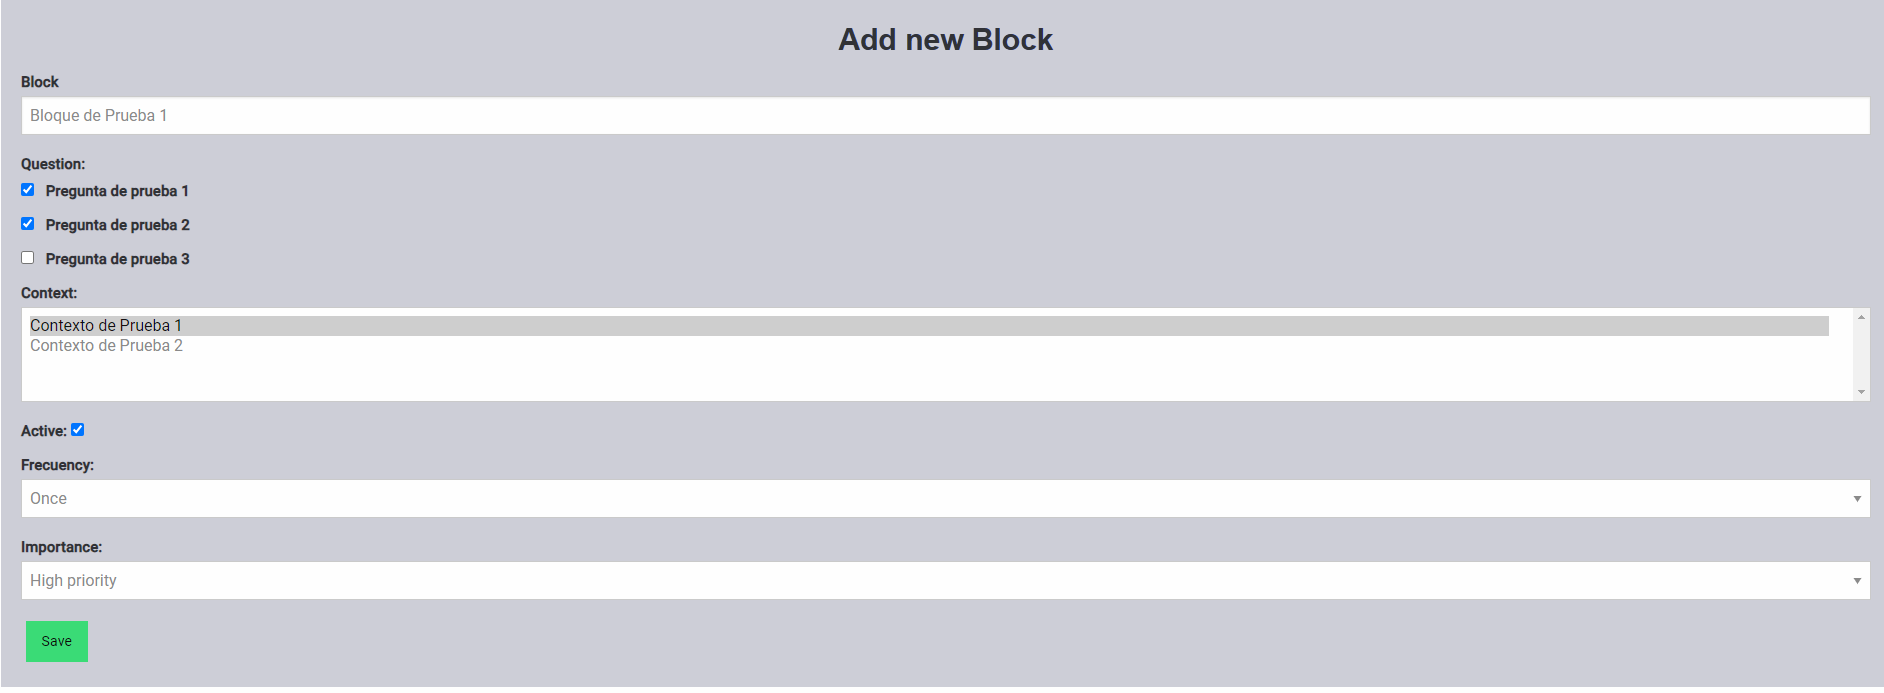
\includegraphics[width=1\textwidth]{imagenes/add_bloque_a1.png}
    \caption{ Vista creación de bloques }
    \label{fig:creacion-bloques}
\end{figure}\vspace{0.5cm}

He creado dos bloques para este ejemplo, como se ve en la \textit{\hyperref[fig:contextos-creados]{figura A.6}}. Uno con las dos primeras preguntas y el primer contexto. Y otro con la última pregunta y otro contexto.  

\begin{figure}[!ht]
    \centering
    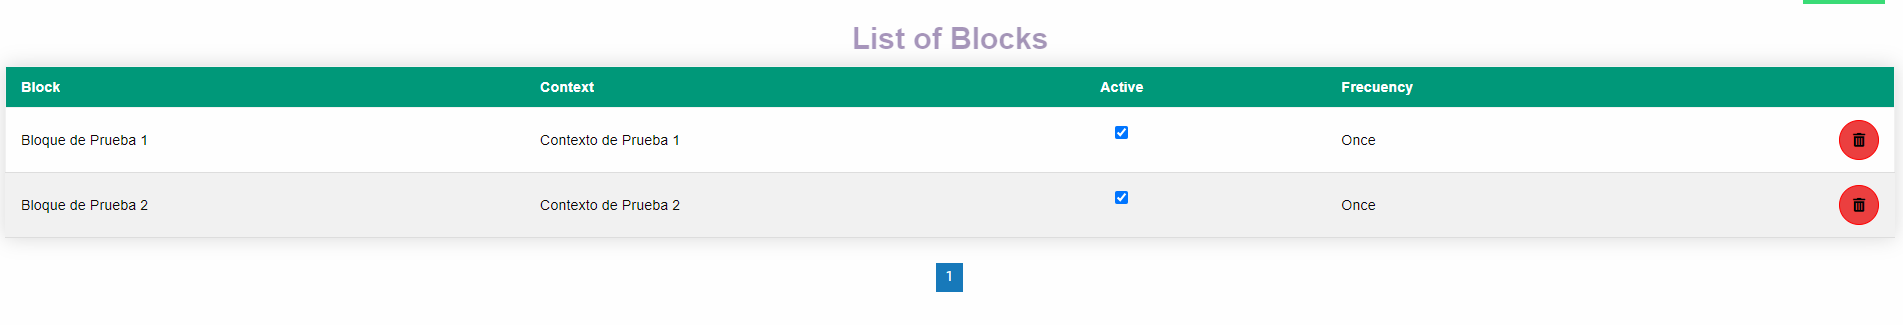
\includegraphics[width=1\textwidth]{imagenes/list_bloques_a.png}
    \caption{ Vista listado de bloques }
    \label{fig:creacion_contexto}
\end{figure}


\subsection{Respondiendo al cuestionario}

Una vez hecho esto, ya podemos pasar a hablar con el bot. Nos dirigimos al chat de Telegram y empezamos la conversación. 

\begin{figure}[!ht]
    \centering
    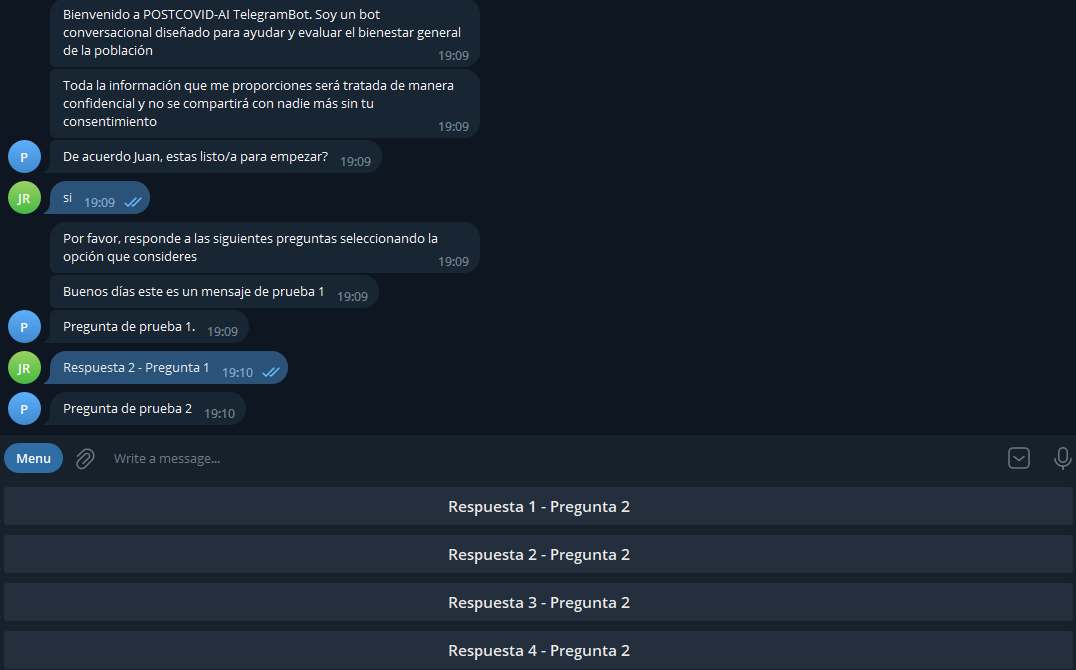
\includegraphics[width=1\textwidth]{imagenes/pregunta_prueba1_a.png}
    \caption{ Cuestionario bloque 1 }
    \label{fig:cuestionario1}
\end{figure}\vspace{0.5cm}

Como se observa en la \textit{\hyperref[fig:cuestionario1]{figura A.7}} el bot detecta que tenemos preguntas pendientes y realiza el cuestionario. Empieza realizando las preguntas asociadas al bloque 1. Primeramente muestra uno de los mensajes del contexto y realiza la primera pregunta, respondemos y realiza la segunda con sus respuestas correspondientes. 

\begin{figure}[!ht]
    \centering
    
\includegraphics[width=1\textwidth]{imagenes/pregunta_prueba2_a.png}
    \caption{ Cuestionario bloque 2 }
    \label{fig:cuestionario2}
\end{figure}\vspace{0.5cm}

Luego, hace lo mismo con el bloque 2 que en este caso solo tenía una pregunta y como se ve en la \textit{\hyperref[fig:cuestionario2]{figura A.8}} el bot nos dice que ya hemos respondido los cuestionarios pendientes. 

\subsection{Administración de Respuestas}

Finalmente, volvemos a la aplicación y esta vez nos dirigimos al último apartado de respuestas. Podemos ver en la \textit{\hyperref[fig:listado_respuestas]{figura A.9}} que se han generado las repuestas a la preguntas que hemos respondido. 

\begin{figure}[!ht]
    \centering
    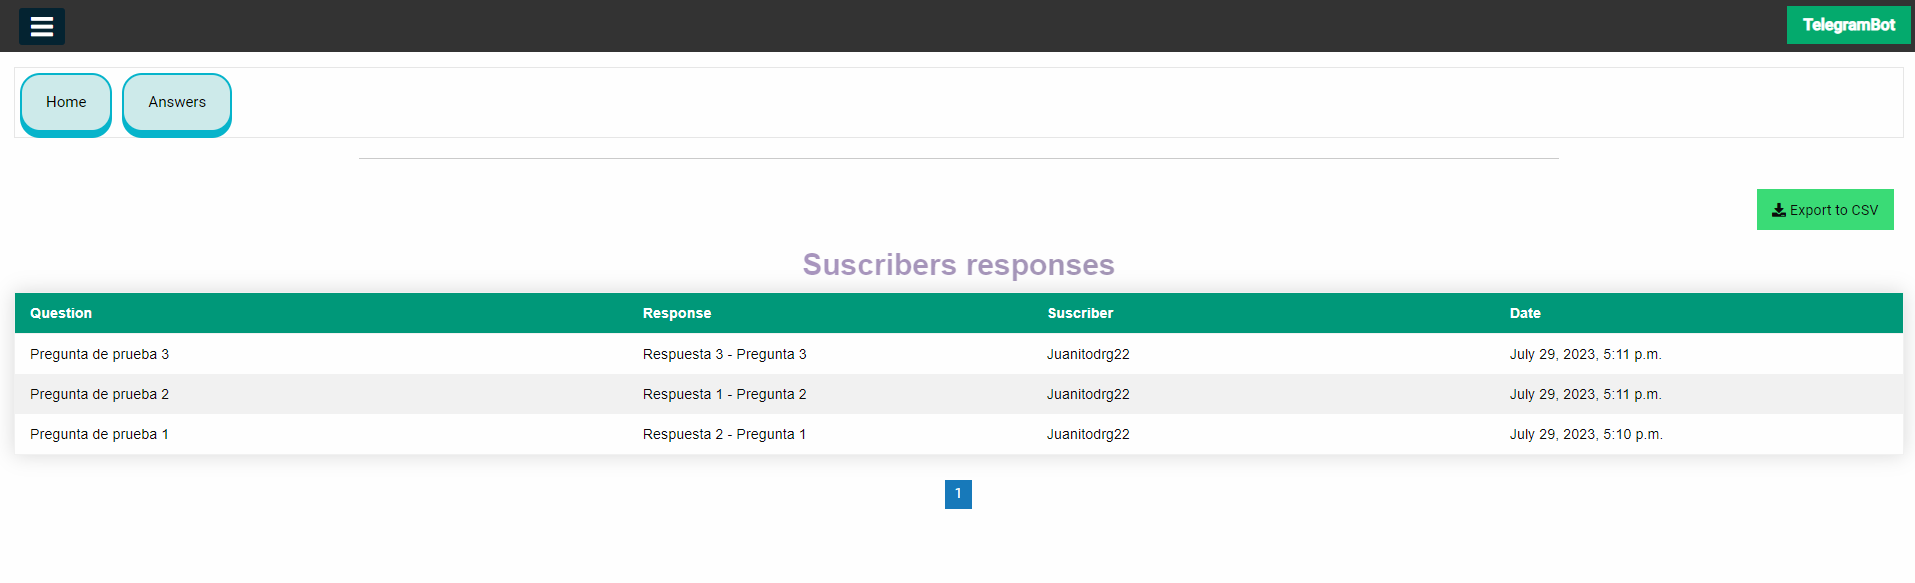
\includegraphics[width=1\textwidth]{imagenes/list_respuestas_a.png}
    \caption{ Vista listado de respuestas }
    \label{fig:listado_respuestas}
\end{figure}\vspace{0.5cm}

Si clicamos en el botón de exportar a CSV nos descarga un archivo que contiene ordenado por columnas la información a las respuestas proporcionadas \textit{\hyperref[fig:respuestas-csv]{(figura A.10)}}. 

\begin{figure}[!ht]
    \centering
    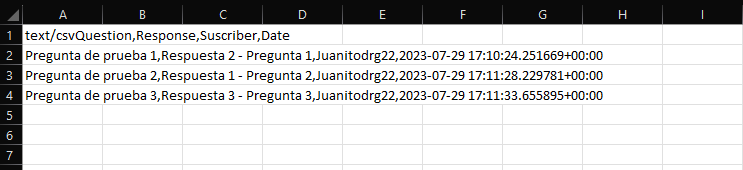
\includegraphics[width=1\textwidth]{imagenes/respuestas_csv_a.png}
    \caption{ Respuestas CSV }
    \label{fig:respuestas-csv}
\end{figure}\vspace{0.5cm}
%
%%\chapter{Conclusiones y Trabajos Futuros}
%
%
\nocite{*}
%\bibliography{bibliografia}\addcontentsline{toc}{chapter}{Bibliografía}
%\bibliographystyle{miunsrturl}
\printbibliography

%
%\appendix
%\input{apendices/manual_usuario/manual_usuario}
%%\input{apendices/paper/paper}
%\input{glosario/entradas_glosario}
% \addcontentsline{toc}{chapter}{Glosario}
% \printglossary


\chapter*{}
\thispagestyle{empty}

\end{document}
